\documentclass[ignorenonframetext,compress]{beamer}
\setbeamertemplate{caption}[numbered]
\setbeamertemplate{caption label separator}{: }
\setbeamercolor{caption name}{fg=normal text.fg}
\beamertemplatenavigationsymbolsempty
\usepackage{lmodern}
\usepackage{amssymb,amsmath}
\usepackage{ifxetex,ifluatex}
\usepackage{fixltx2e} % provides \textsubscript
\ifnum 0\ifxetex 1\fi\ifluatex 1\fi=0 % if pdftex
\usepackage[T1]{fontenc}
\usepackage[utf8]{inputenc}
\else % if luatex or xelatex
\ifxetex
\usepackage{mathspec}
\else
\usepackage{fontspec}
\fi
\defaultfontfeatures{Ligatures=TeX,Scale=MatchLowercase}
\fi
\usetheme{Singapore}
% use upquote if available, for straight quotes in verbatim environments
\IfFileExists{upquote.sty}{\usepackage{upquote}}{}
% use microtype if available
\IfFileExists{microtype.sty}{%
\usepackage{microtype}
\UseMicrotypeSet[protrusion]{basicmath} % disable protrusion for tt fonts
}{}
\newif\ifbibliography
\usepackage{graphicx,grffile}
\makeatletter
\def\maxwidth{\ifdim\Gin@nat@width>\linewidth\linewidth\else\Gin@nat@width\fi}
\def\maxheight{\ifdim\Gin@nat@height>\textheight0.8\textheight\else\Gin@nat@height\fi}
\makeatother
% Scale images if necessary, so that they will not overflow the page
% margins by default, and it is still possible to overwrite the defaults
% using explicit options in \includegraphics[width, height, ...]{}
\setkeys{Gin}{width=\maxwidth,height=\maxheight,keepaspectratio}

% Prevent slide breaks in the middle of a paragraph:
\widowpenalties 1 10000
\raggedbottom

\AtBeginPart{
\let\insertpartnumber\relax
\let\partname\relax
\frame{\partpage}
}
\AtBeginSection{
\ifbibliography
\else
\let\insertsectionnumber\relax
\let\sectionname\relax
\frame{\sectionpage}
\fi
}
\AtBeginSubsection{
\let\insertsubsectionnumber\relax
\let\subsectionname\relax
\frame{\subsectionpage}
}

\setlength{\parindent}{0pt}
\setlength{\parskip}{6pt plus 2pt minus 1pt}
\setlength{\emergencystretch}{3em}  % prevent overfull lines
\providecommand{\tightlist}{%
\setlength{\itemsep}{0pt}\setlength{\parskip}{0pt}}
\setcounter{secnumdepth}{0}
\usepackage{graphicx}
\usepackage{array}
\usepackage{tabularx}                                             % table environment providing flexibility
\usepackage{caption}                                              % for creating captions  
\usepackage{longtable}                                            % allows tables to span multiple pages
\usepackage{rotating}                                             % allows for sideways tables
\usepackage{float}                                                % floating environments; may not need in rmarkdown
\usepackage{placeins}                                             % keeps floats from moving
\usepackage{indentfirst}                                          % indents first paragraph of a section
\usepackage{mdwtab}                                               % continued float multi-page figure
\usepackage{enumerate}                                            % create lists
\usepackage{hyperref}                                             % highlight cross references
\usepackage{enumitem}                                             % numbered lists
\usepackage{upquote}                                              % produce grave accent in latex
\usepackage{verbatim}                                             % produces verbatim results
\usepackage{fancyvrb}                                             % verbatim in a box
\usepackage{textcomp}                                             % fixes error with packages interfering
\usepackage{cmap}                                                 % fix mapping characters to unicode
\usepackage{appendixnumberbeamer}
\usepackage{lscape}

\setbeamersize{text margin left=0.1in}
\setbeamersize{text margin right=0.1in}

\definecolor{pageCol}{rgb}{0.5,0.5,1.0}

\usepackage{tikz}                                                   % used in background


\usebackgroundtemplate{
  \tikz[overlay,remember picture] 
  \node[opacity=0.3, at=(current page.south east),anchor=south east,inner sep=0pt] {
    
\includegraphics[height=0.5in]{noaalogo.jpg}};
}

\setbeamertemplate{footline}
{
  \begin{beamercolorbox}[wd=.05\paperwidth,ht=0ex,dp=0ex,left]{framenumber in head/foot}%
    \insertframenumber/\inserttotalframenumber
    
  \end{beamercolorbox}%
}
\setbeamercolor{footline}{fg=pageCol}


\newcounter{saveenumi}

%Itemize with bullet
\setbeamertemplate{itemize item}{$\circ$}

%To get two columns
\def\begincols{\begin{columns}}
\def\begincol{\begin{column}}
\def\endcol{\end{column}}
\def\endcols{\end{columns}}

\title{California Scorpionfish 2017 Stock Assessment}
\author{Melissa H Monk\(^1\), \and Xi He\(^1\), \and John Budrick\(^2\)}
\institute{\(^1\)Southwest Fisheries Science Center \and \(^2\)California Department of Fish and Wildlife}
\date{STAR Panel meeing July 24-28, 2017}

\begin{document}
\frame{\titlepage}

\begin{frame}
\tableofcontents[hideallsubsections]
\end{frame}

\begin{frame}

\end{frame}

\section{Background}\label{background}

\begin{frame}{California scorpionfish (\emph{Scorpaena guttata})}

\begin{itemize} 
 \item[$\circ$] Most common species of \emph{Scorpaena} on the U.S. West Coast, more species in Mexico
 \item[$\circ$] Venomous dorsal, anal and pelvic spines
 \item[$\circ$] Demersal, found over both hard and soft bottom (prefer \emph{new} structure)
 \item[$\circ$] Exhibit aggregating behavior (spawning and non-spawning aggregations)  
\end{itemize}

\centering
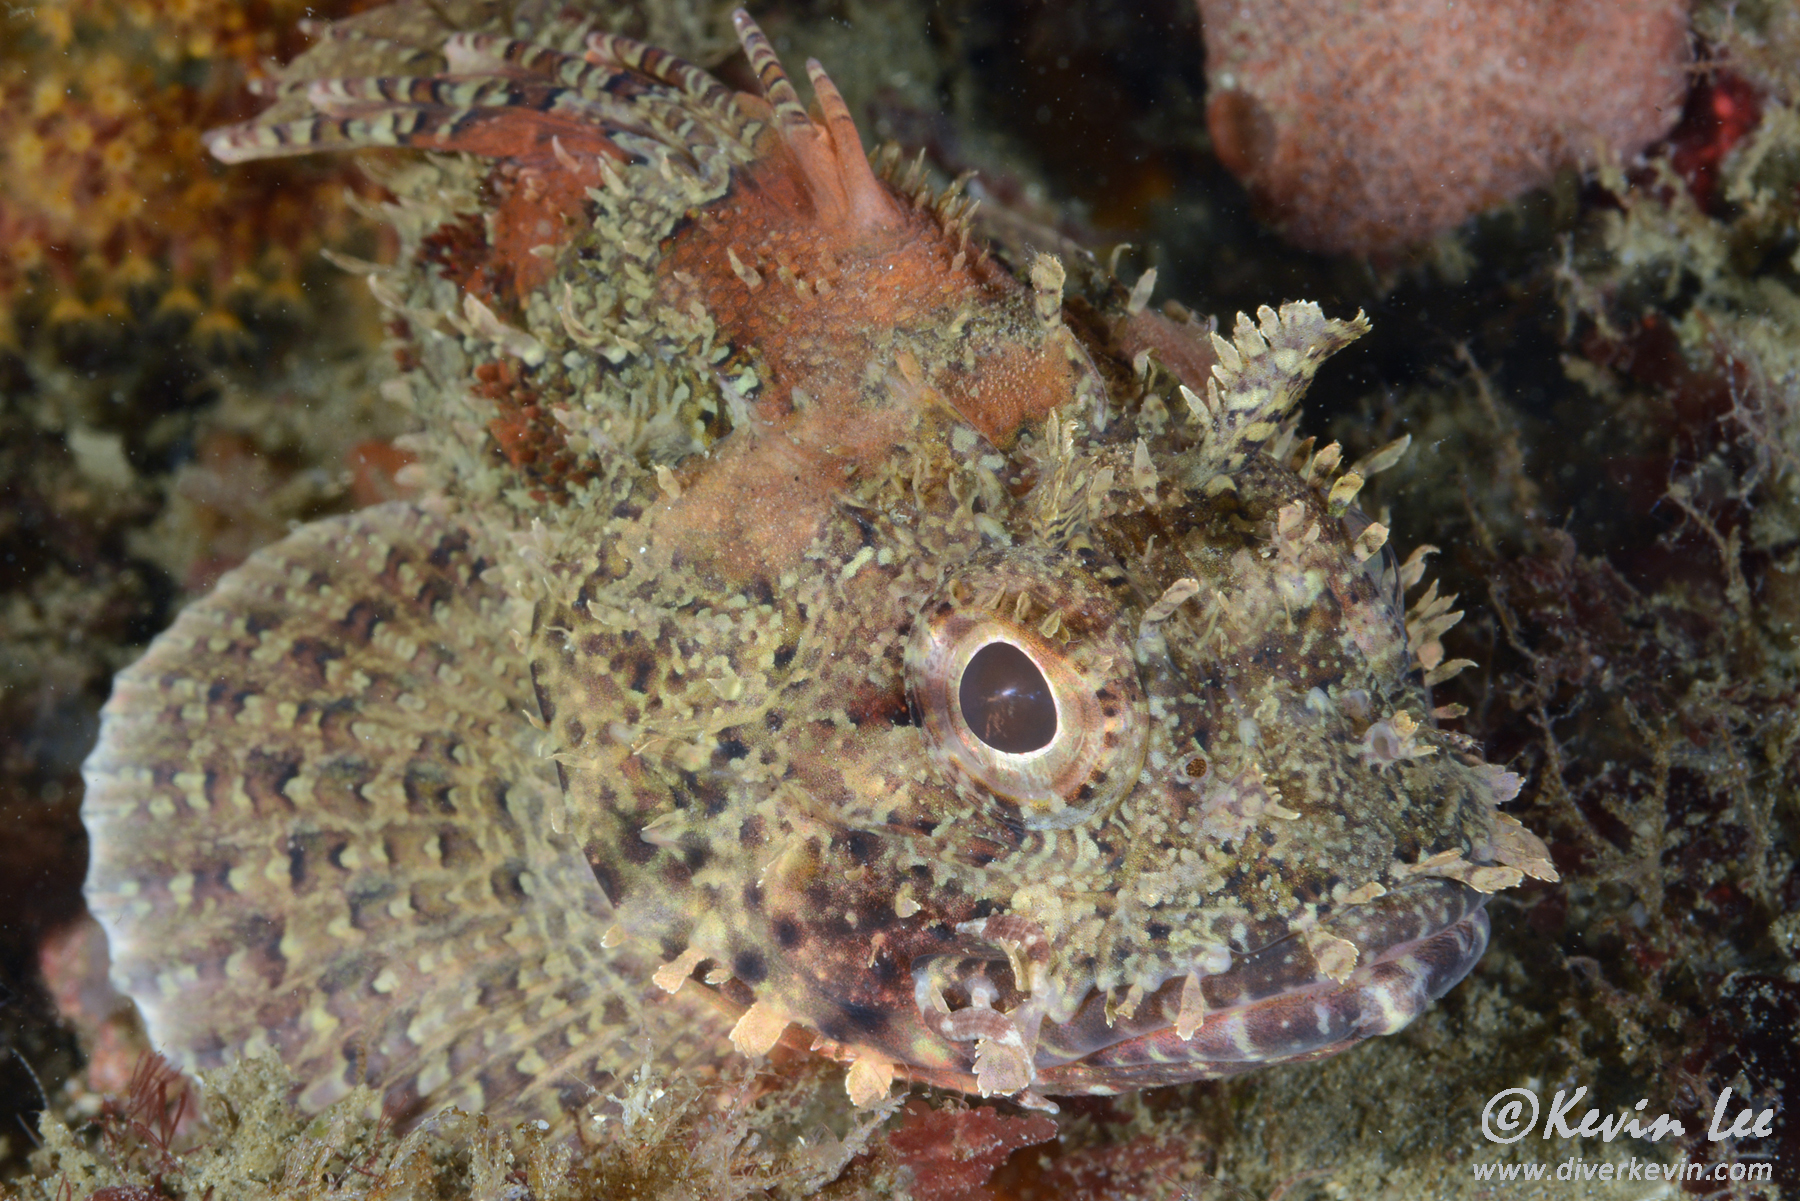
\includegraphics[width=.5\textwidth]{cover_photo}

\end{frame}

\begin{frame}{Early Life History}

\begin{itemize} 
\item[$\circ$] Migration to spawning grounds, exhibit explosive breeding behavior just before dawn
\item[$\circ$] External fertilization, females produce hollow gelatenous single-layer floating egg matrix
\item[$\circ$] Eggs hatch after about 5 days
\item[$\circ$] Juveniles settle at less than 2cm 
\end{itemize}

\centering
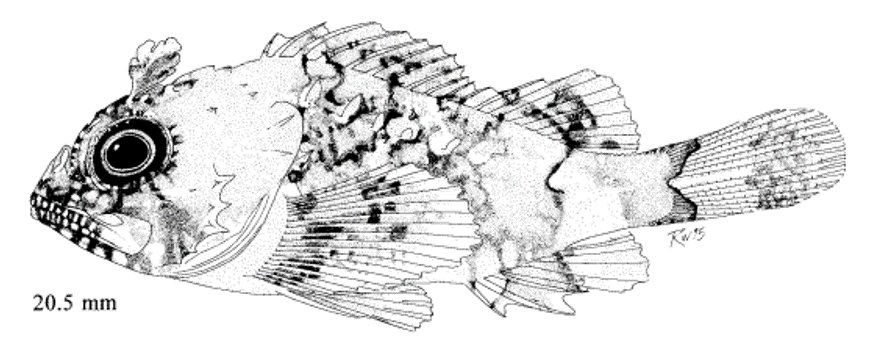
\includegraphics[width=.5\textwidth]{Figures/baby_scorp}

\footnotetext{Line drawning from CalCOFI Atlas 33, pg. 789 Figure 26}

\end{frame}

\begin{frame}{Distribution}

\begin{itemize} 
 \item[$\circ$] Distributed from central California to Punta Eugenia, Baja California Sur, Mexico 
 \item[$\circ$] Rarely observed north of Pt. Conception  
 \item[$\circ$] Observed from the intertidal to 600 ft,  prefer 20-450 ft  
 \item[$\circ$] Proportion of the stock in Mexican waters unknown
\end{itemize}

\end{frame}

\begin{frame}{Distribution}

\end{frame}

\begin{frame}{Stock Assessment Boundary}

\centering
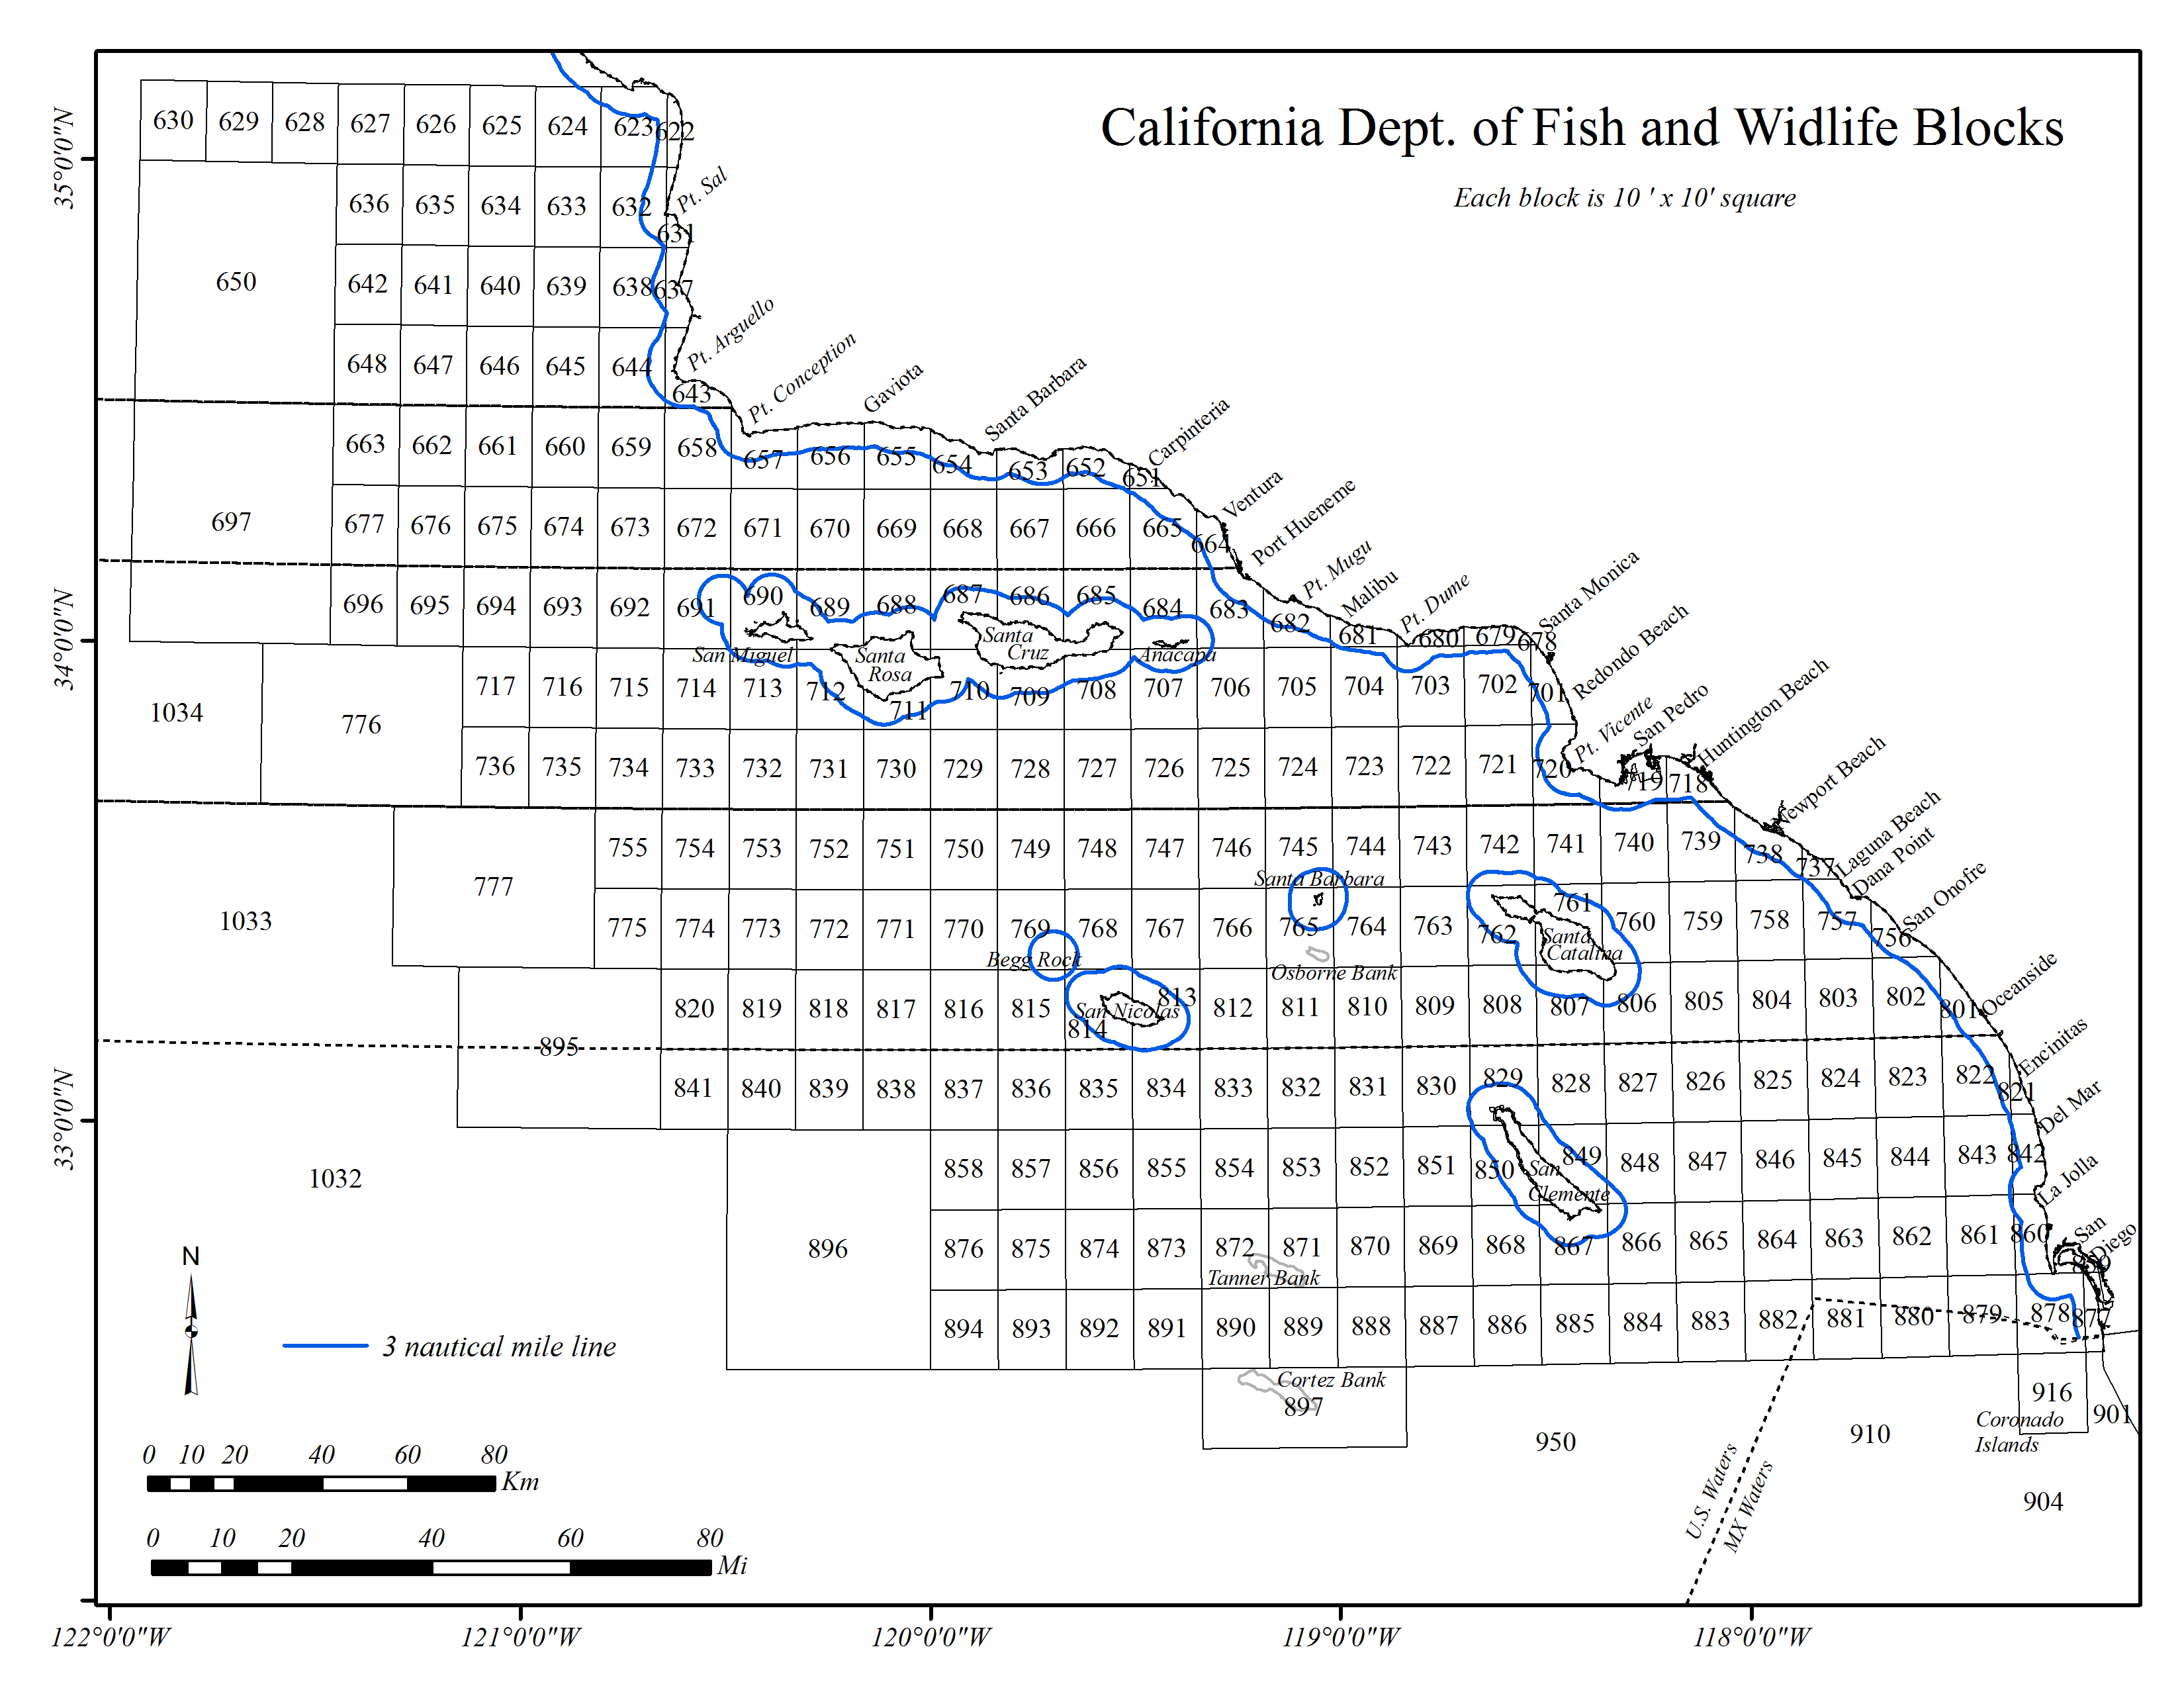
\includegraphics{Figures/assess_region_map.png}

\end{frame}

\begin{frame}{2005 Stock Assessment}

\begin{itemize}
\item[$\circ$] Stock first assessed in 2005
\item[$\circ$] South of Pt. Conception
\item[$\circ$] $M$ fixed at 0.25
\item[$\circ$] $h$ 0.7
\end{itemize}

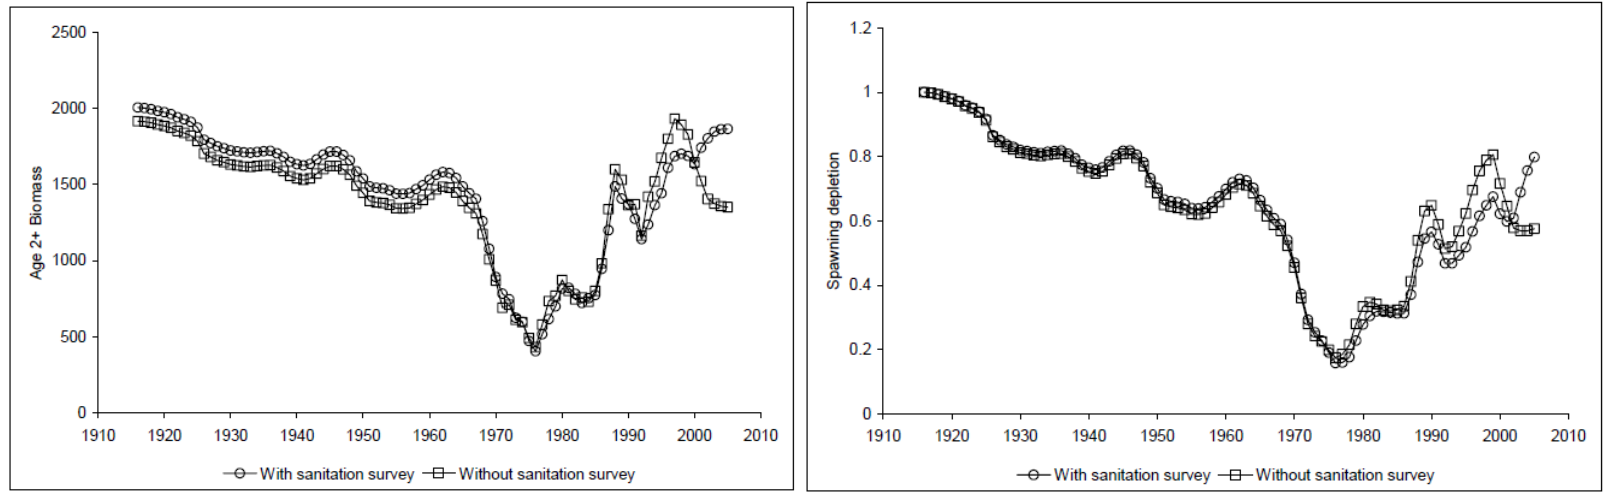
\includegraphics{Figures/2005_bio_depl.png}

\end{frame}

\begin{frame}{2005 Stock Assessment}

\begin{itemize}
\item[$\circ$] Transitioning from the 2005 assessment, an error was found
\item[$\circ$] Harvest rate hit the bounds for the recreational fleet
\item[$\circ$] Not all of the recreational catch was removed
\item[$\circ$] Input vs. estimated catch was not standard output in SS v.1.8
\end{itemize}

\begincols
 \begincol{.4\textwidth}

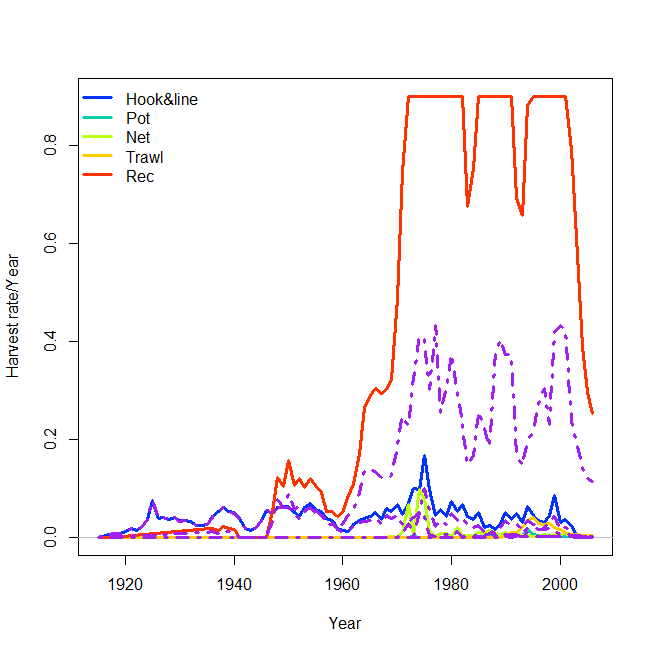
\includegraphics{Figures/bridge_harvestrate.png}

\endcol
 \begincol{.48\textwidth}

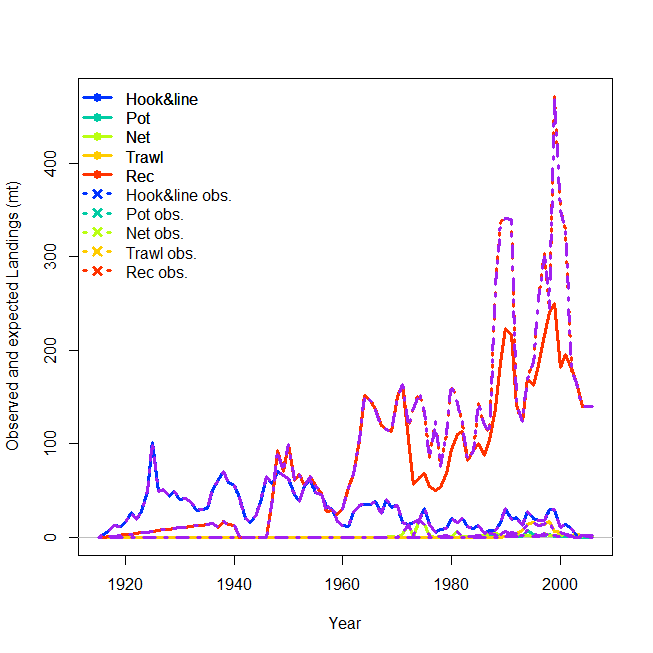
\includegraphics{Figures/bridge_catch.png}

\endcol
\endcols

\end{frame}

\begin{frame}{2005 Stock Assessment}

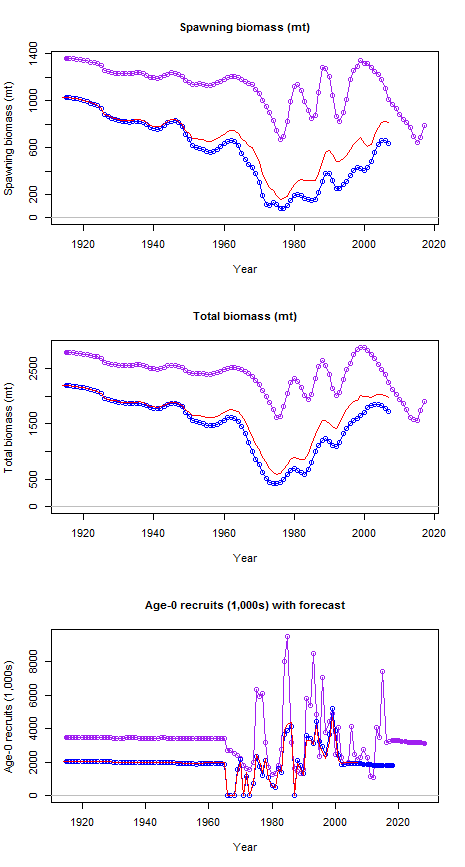
\includegraphics{Figures/bridge_timeseries.png}

\end{frame}

\begin{frame}{2017 Stock Assessment}

\begin{itemize}
\item[$\circ$] One area south of Pt. Conception (all catches from Mexican waters excluded as in 2005)
\end{itemize}

\end{frame}

\subsection{Length-at-age}\label{length-at-age}

\begin{frame}{Length-at-age}

\begincols
 \begincol{.4\textwidth}

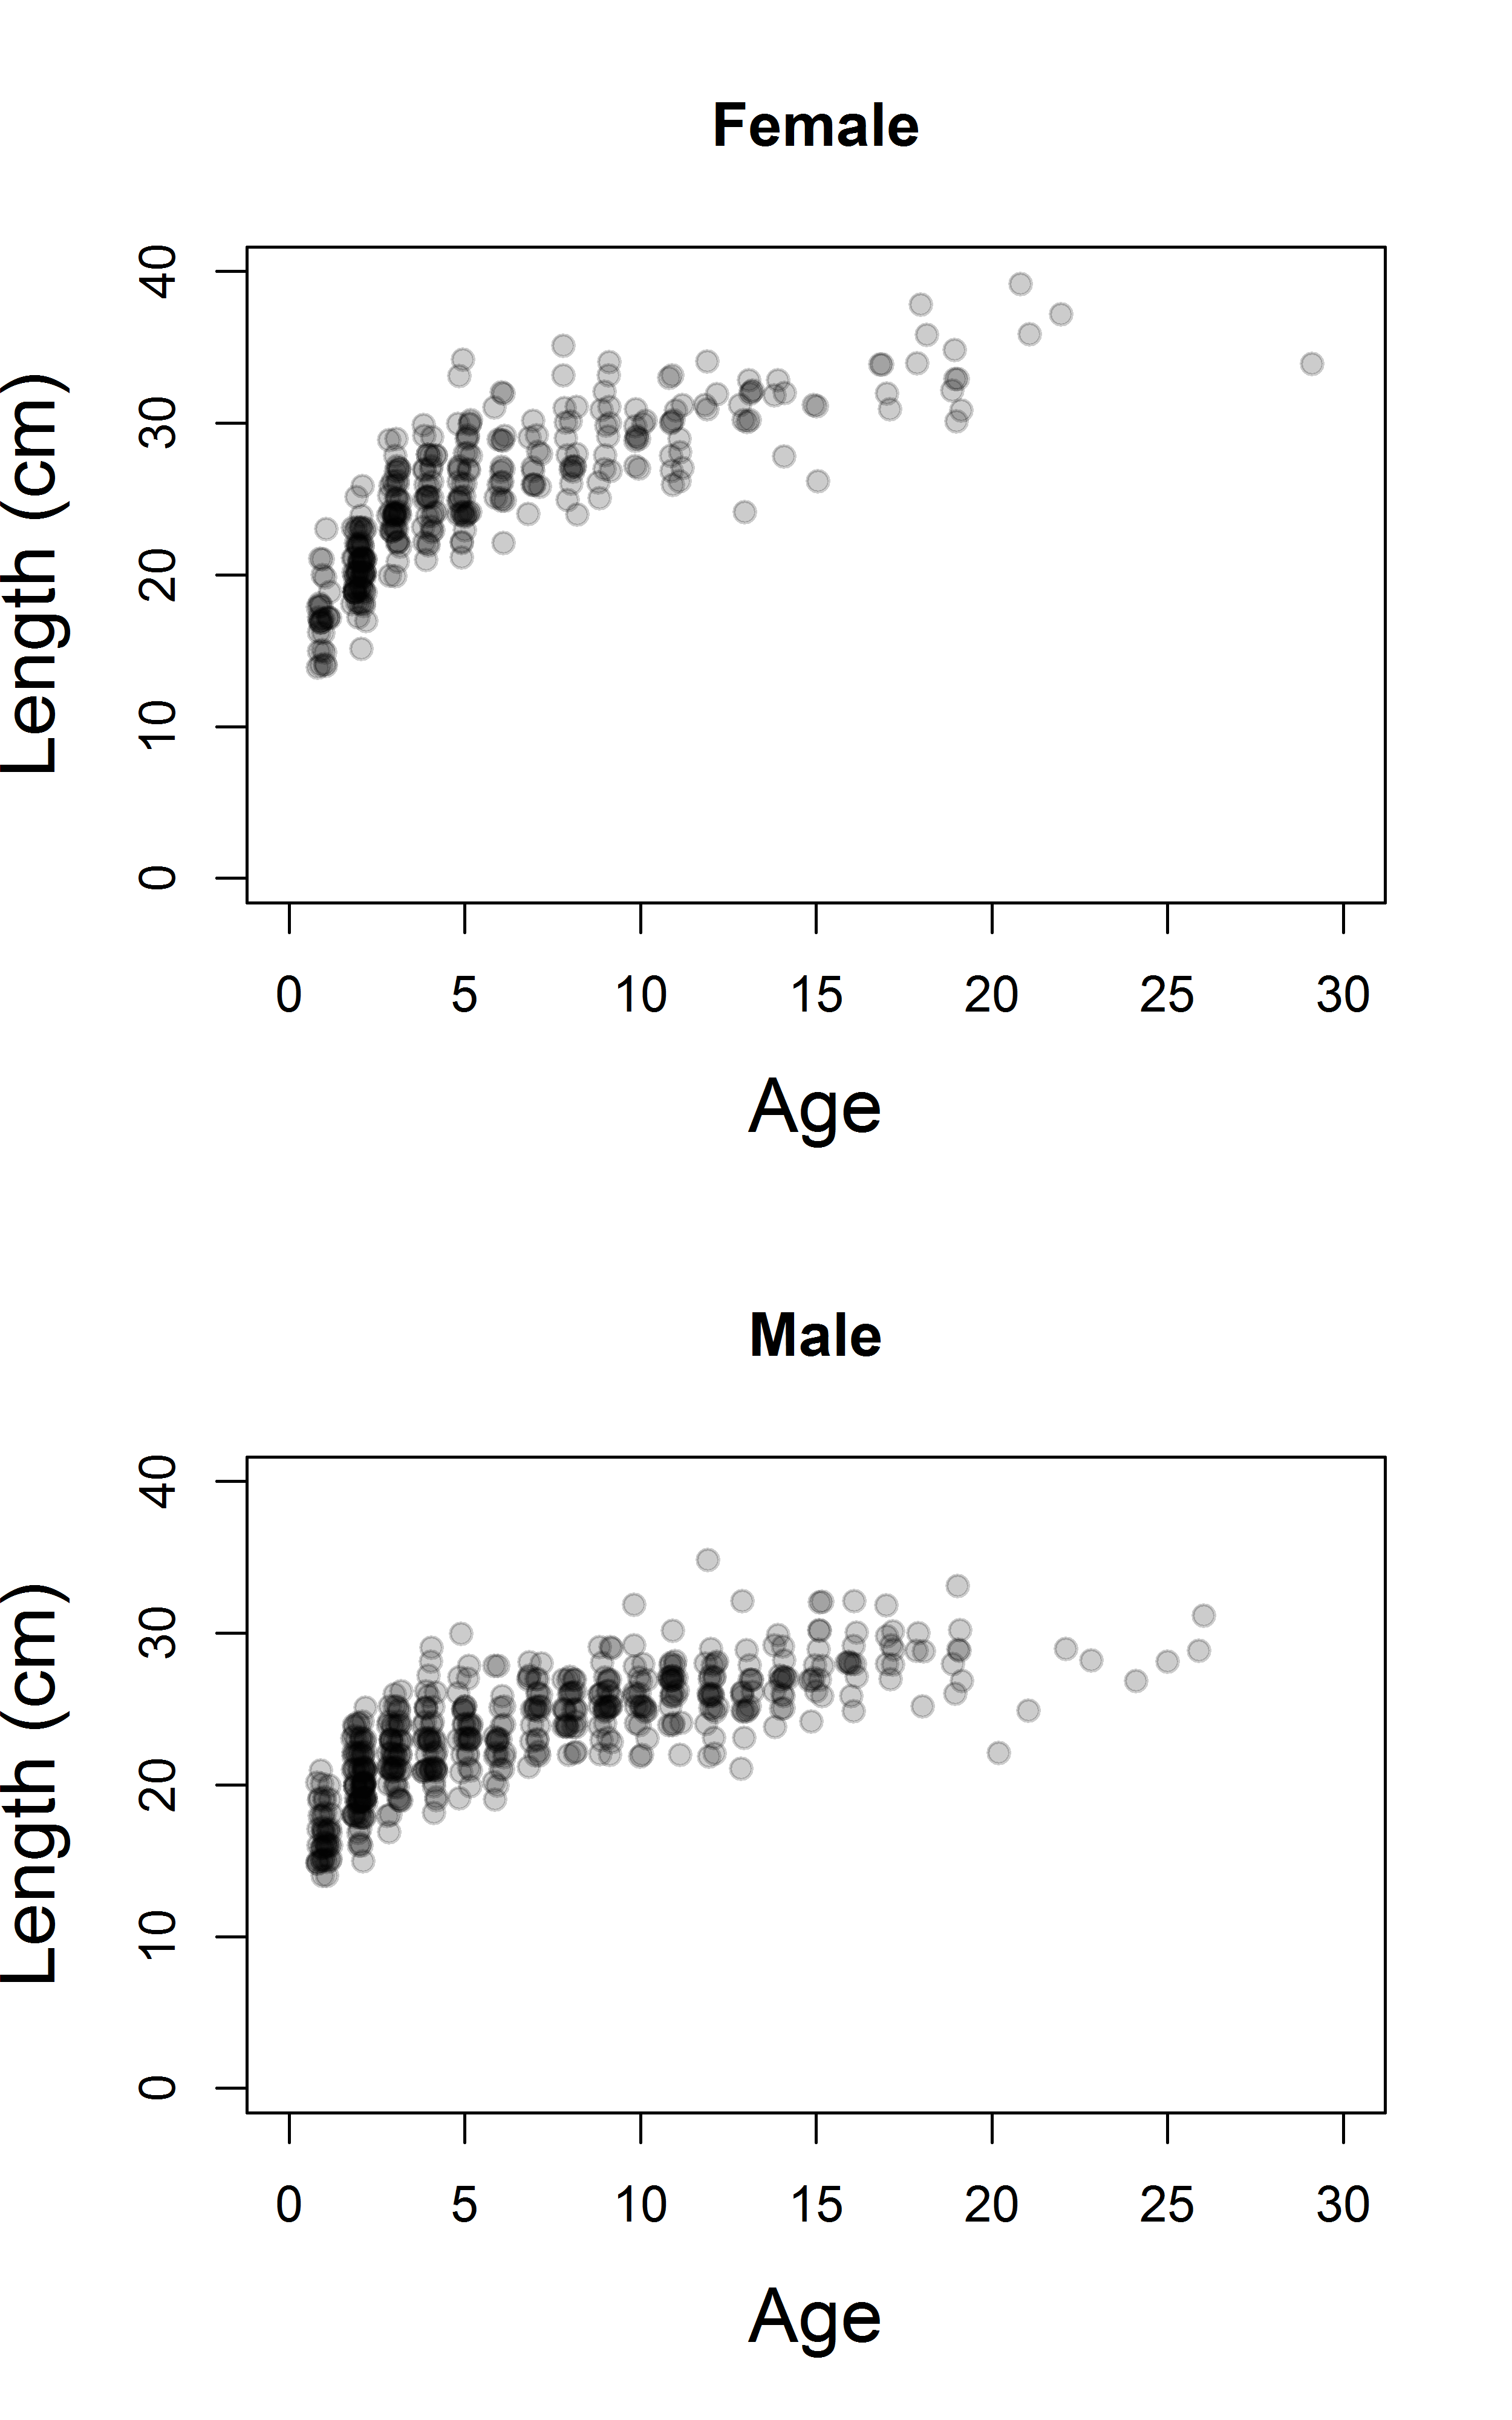
\includegraphics[trim={0 0 0 2cm}, totalheight=0.65\textheight]{Figures/Age_length_bySex.png}

\endcol
 \begincol{.48\textwidth}

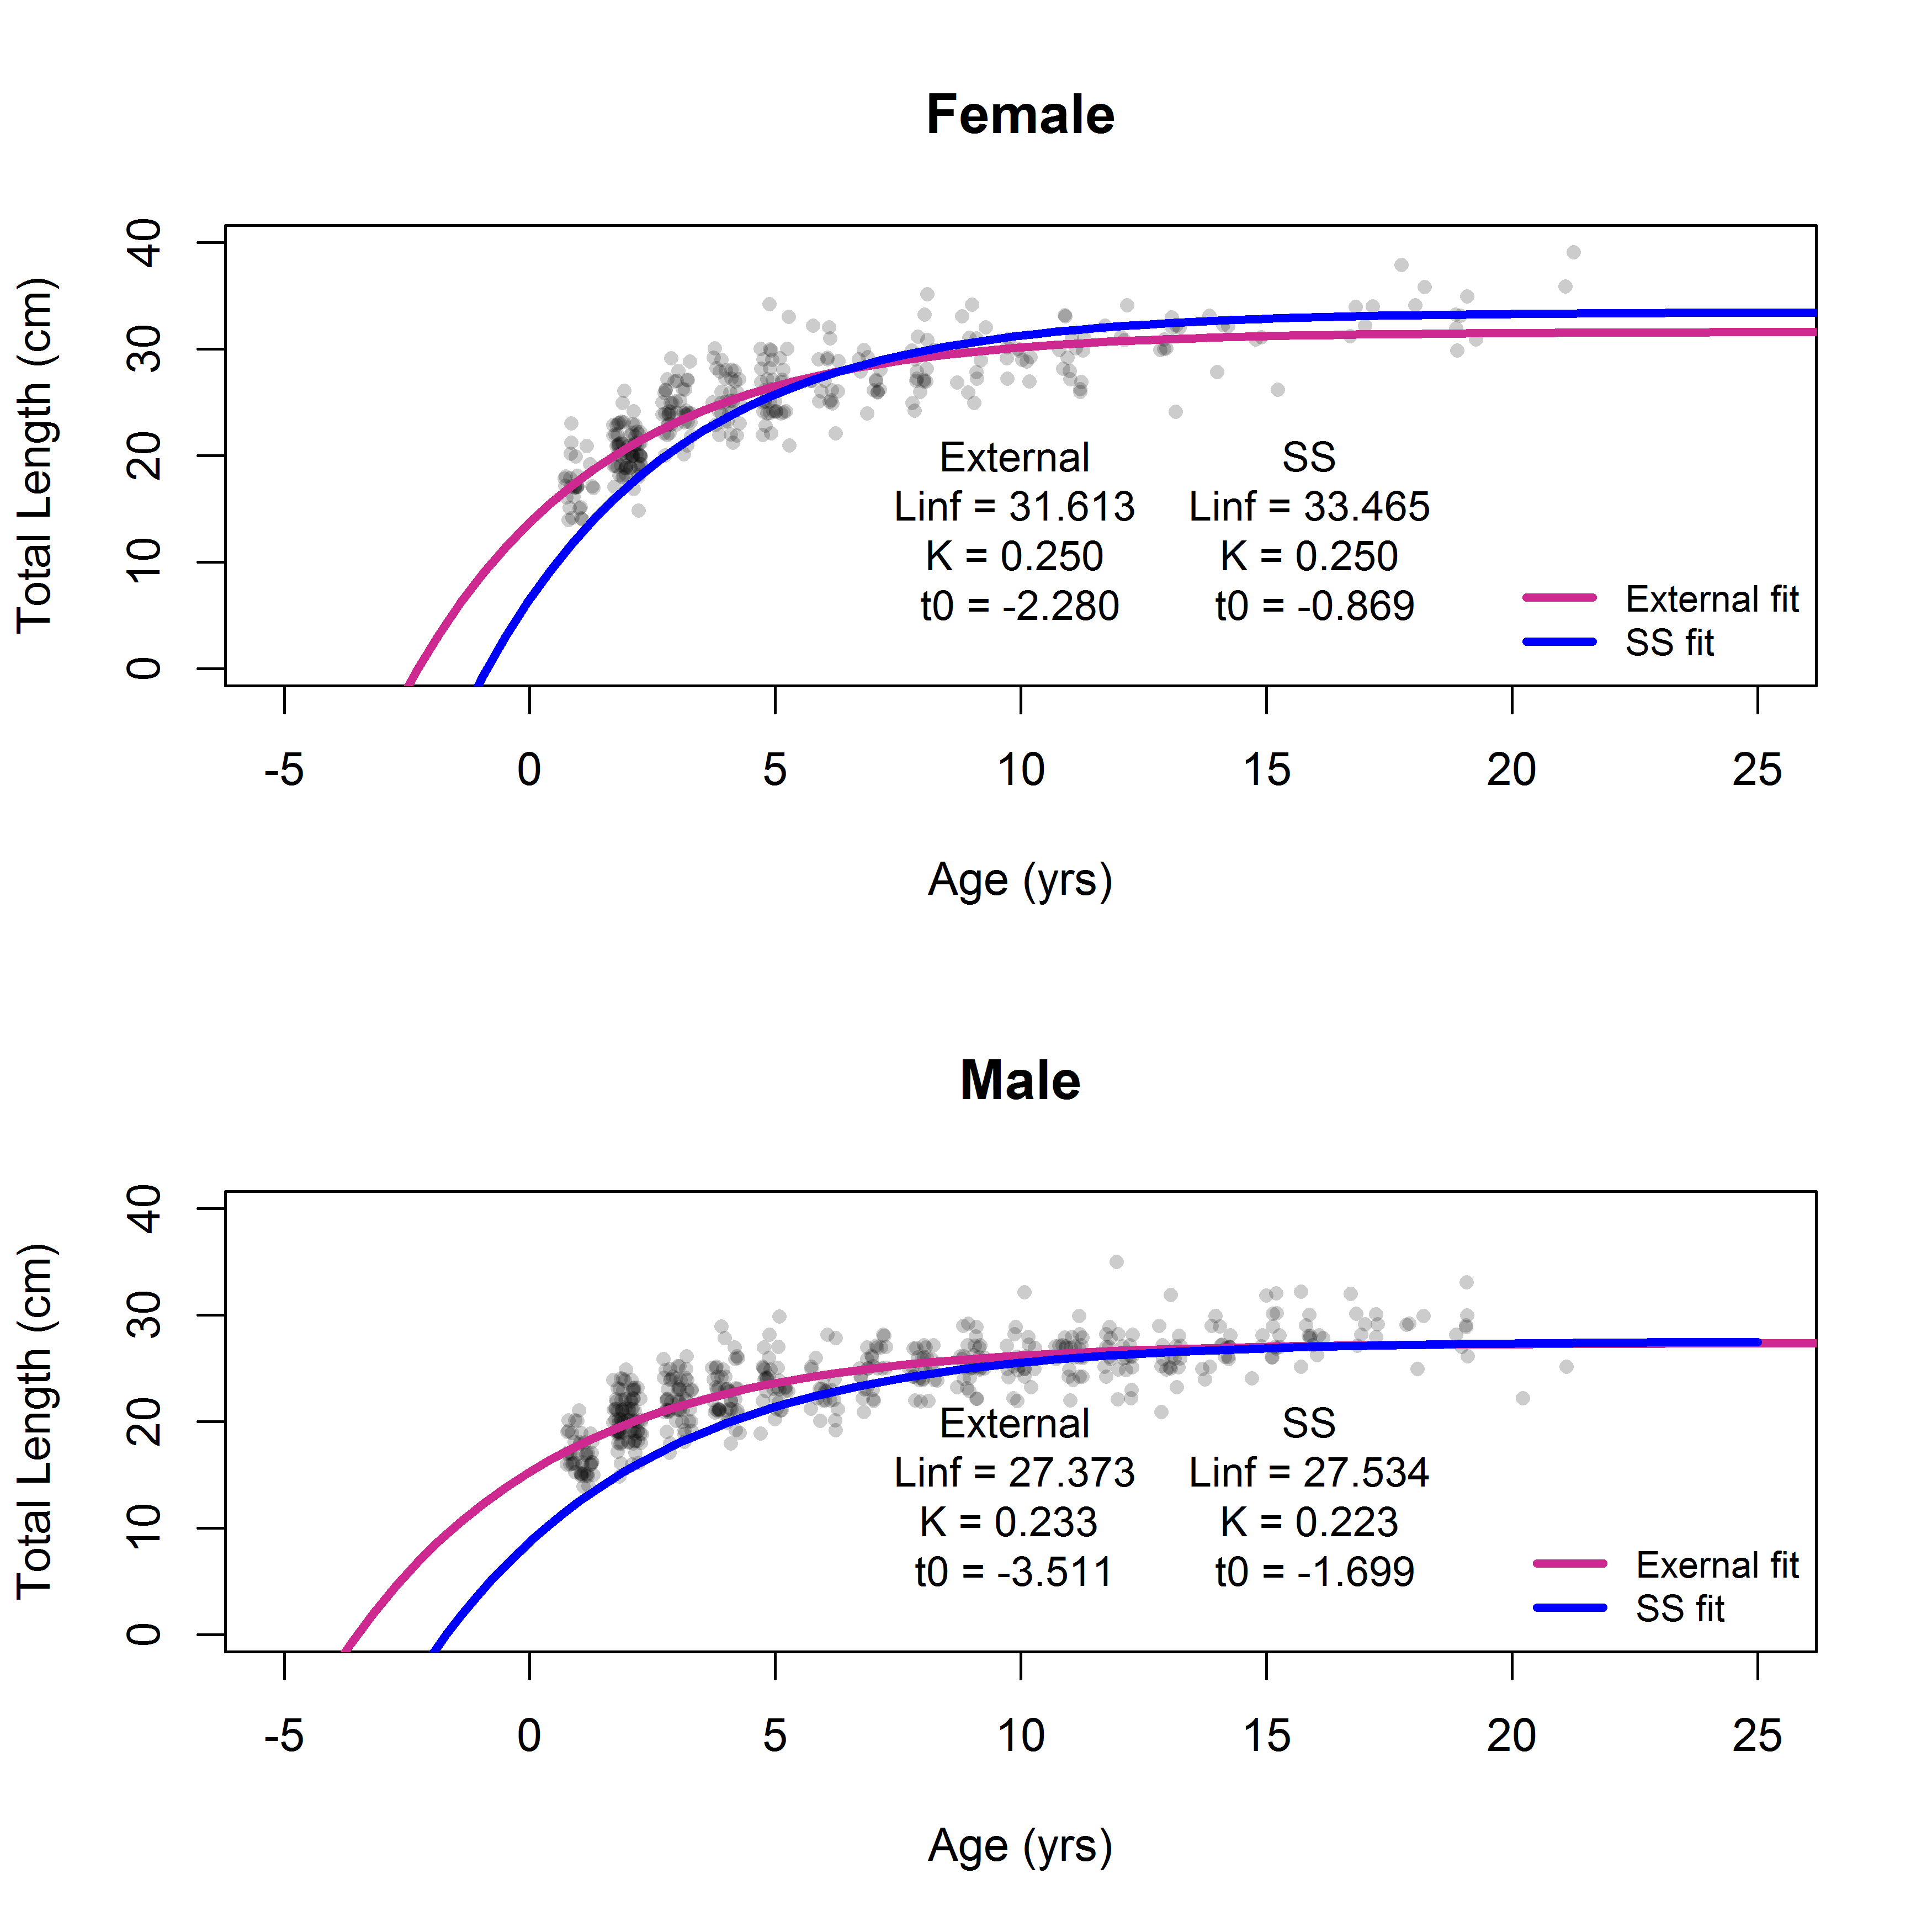
\includegraphics{Figures/vonB_compare.png}

\endcol
\endcols

\end{frame}

\begin{frame}{Length-at-age}

\begincols
 \begincol{.4\textwidth}

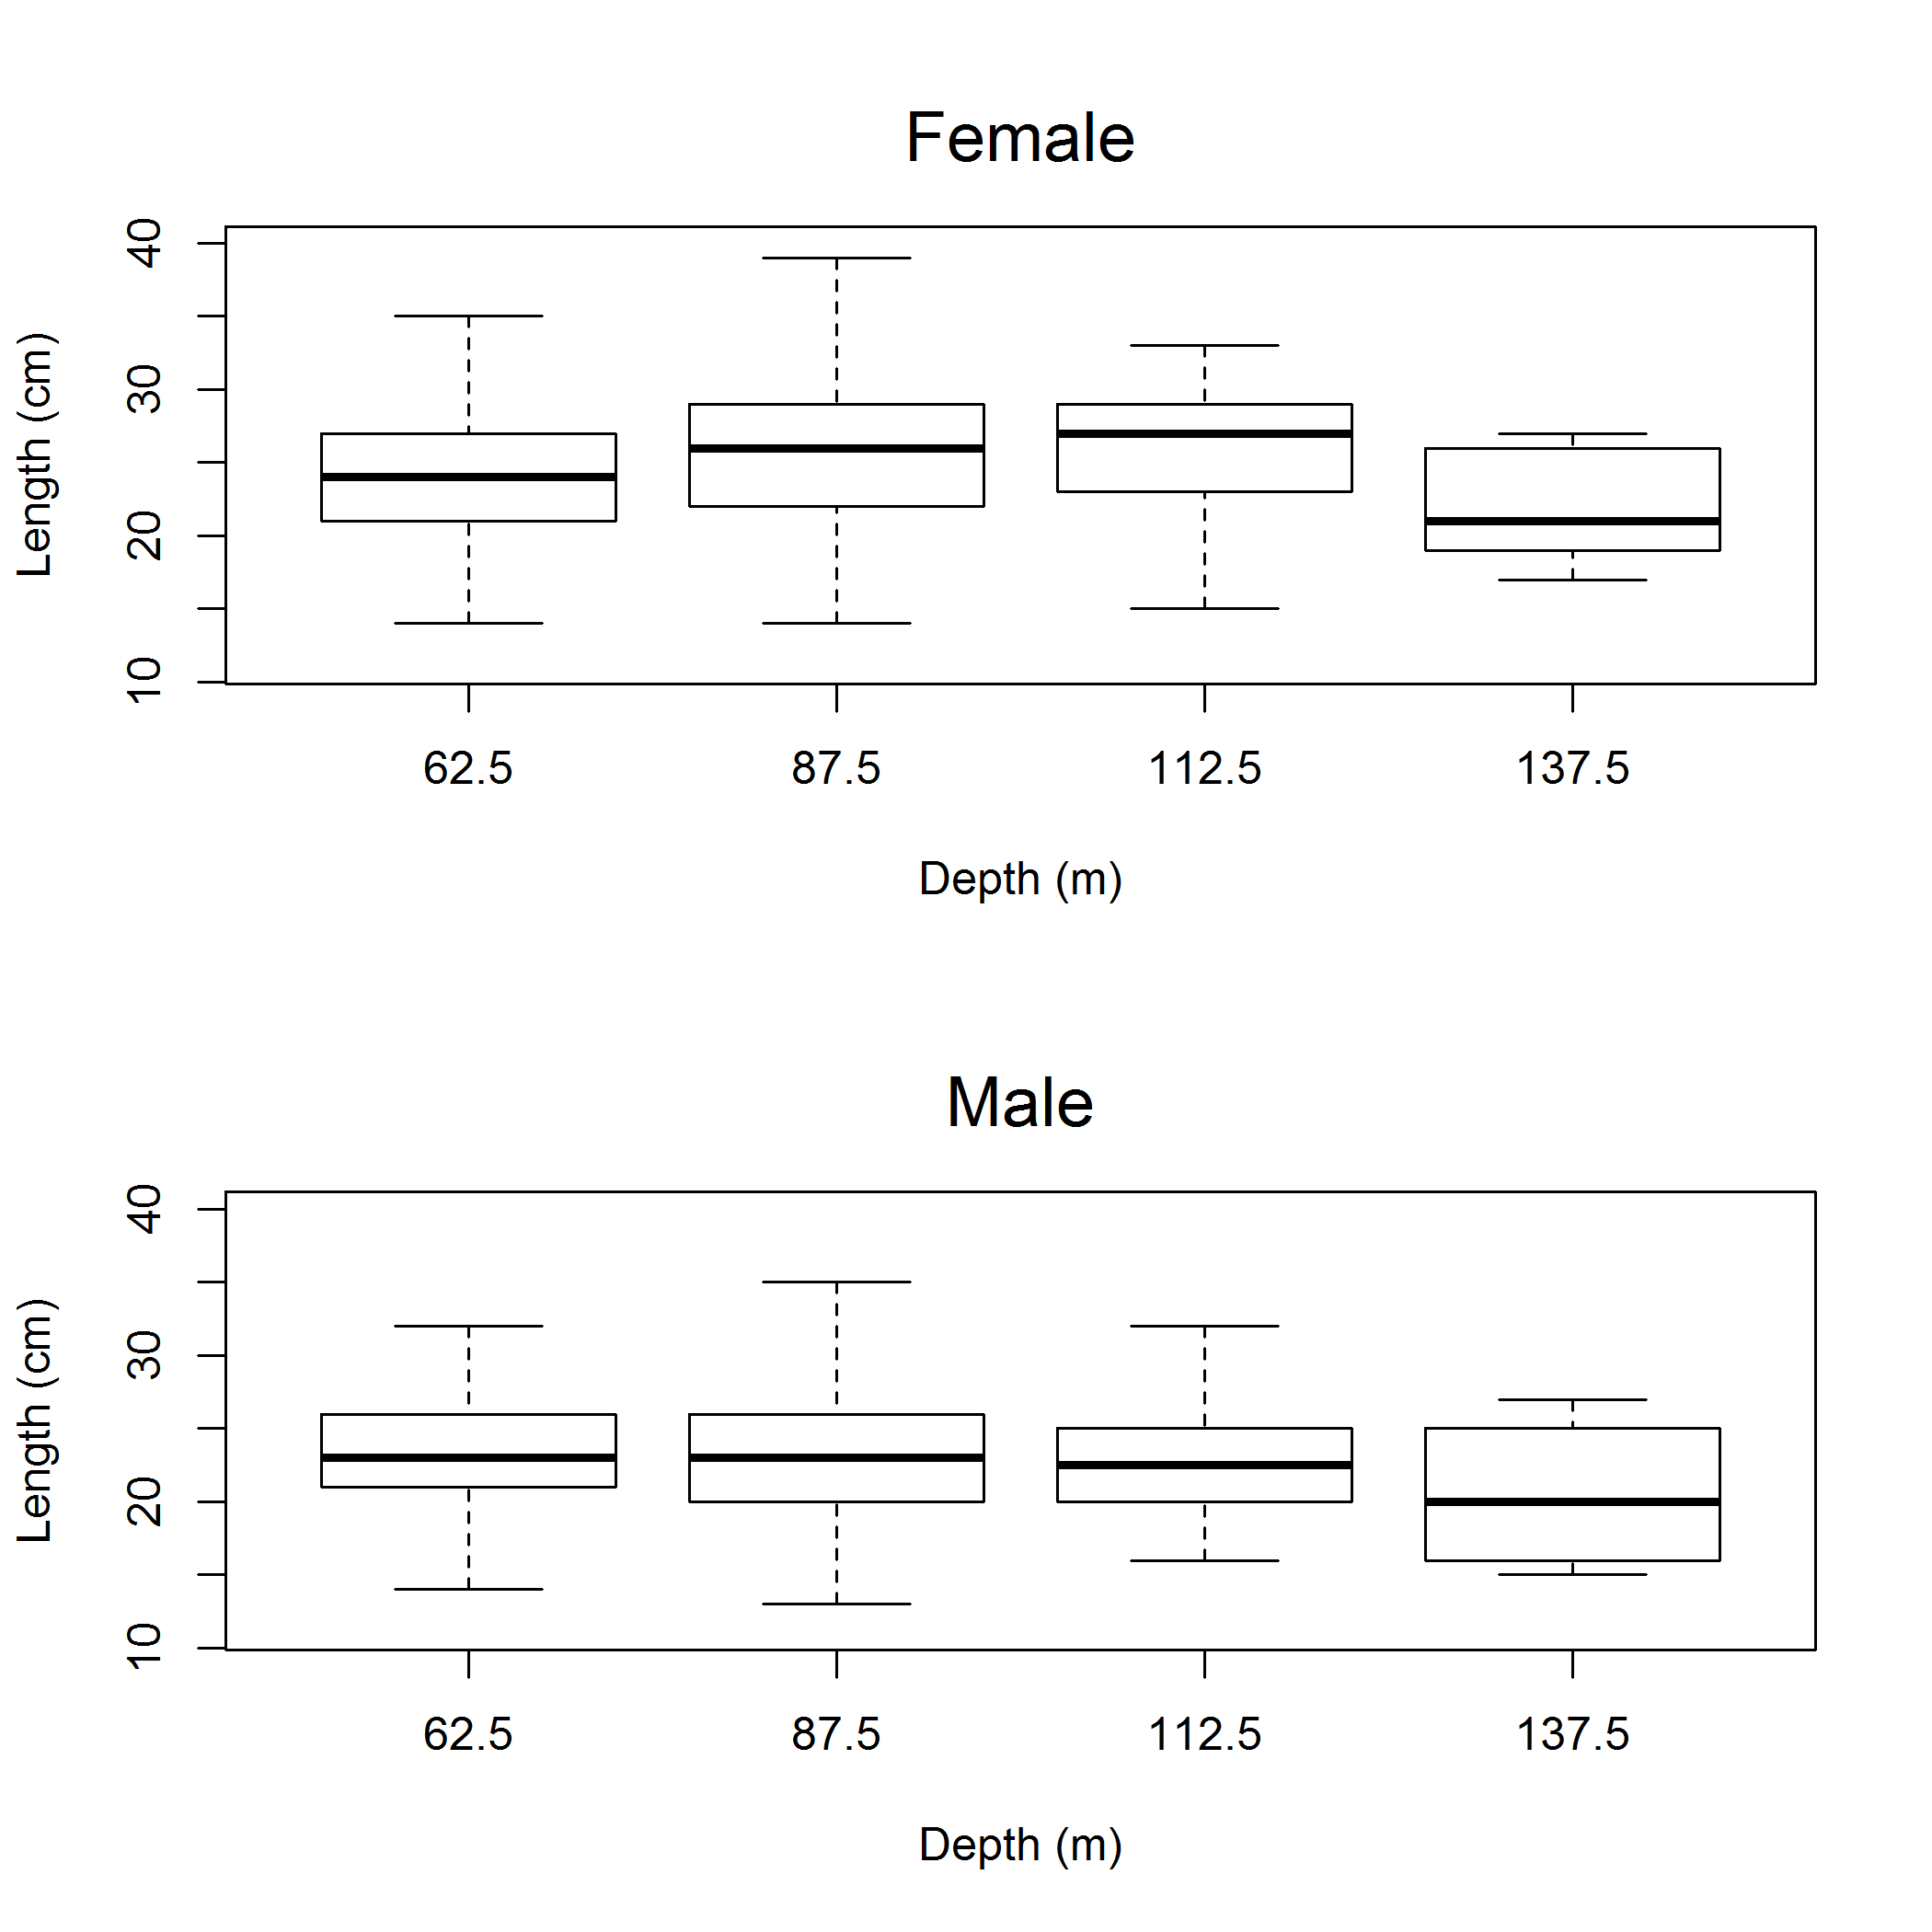
\includegraphics{Figures/NWFSCtrawl_lengthdepth.png}

\endcol
\begincol{.48\textwidth}

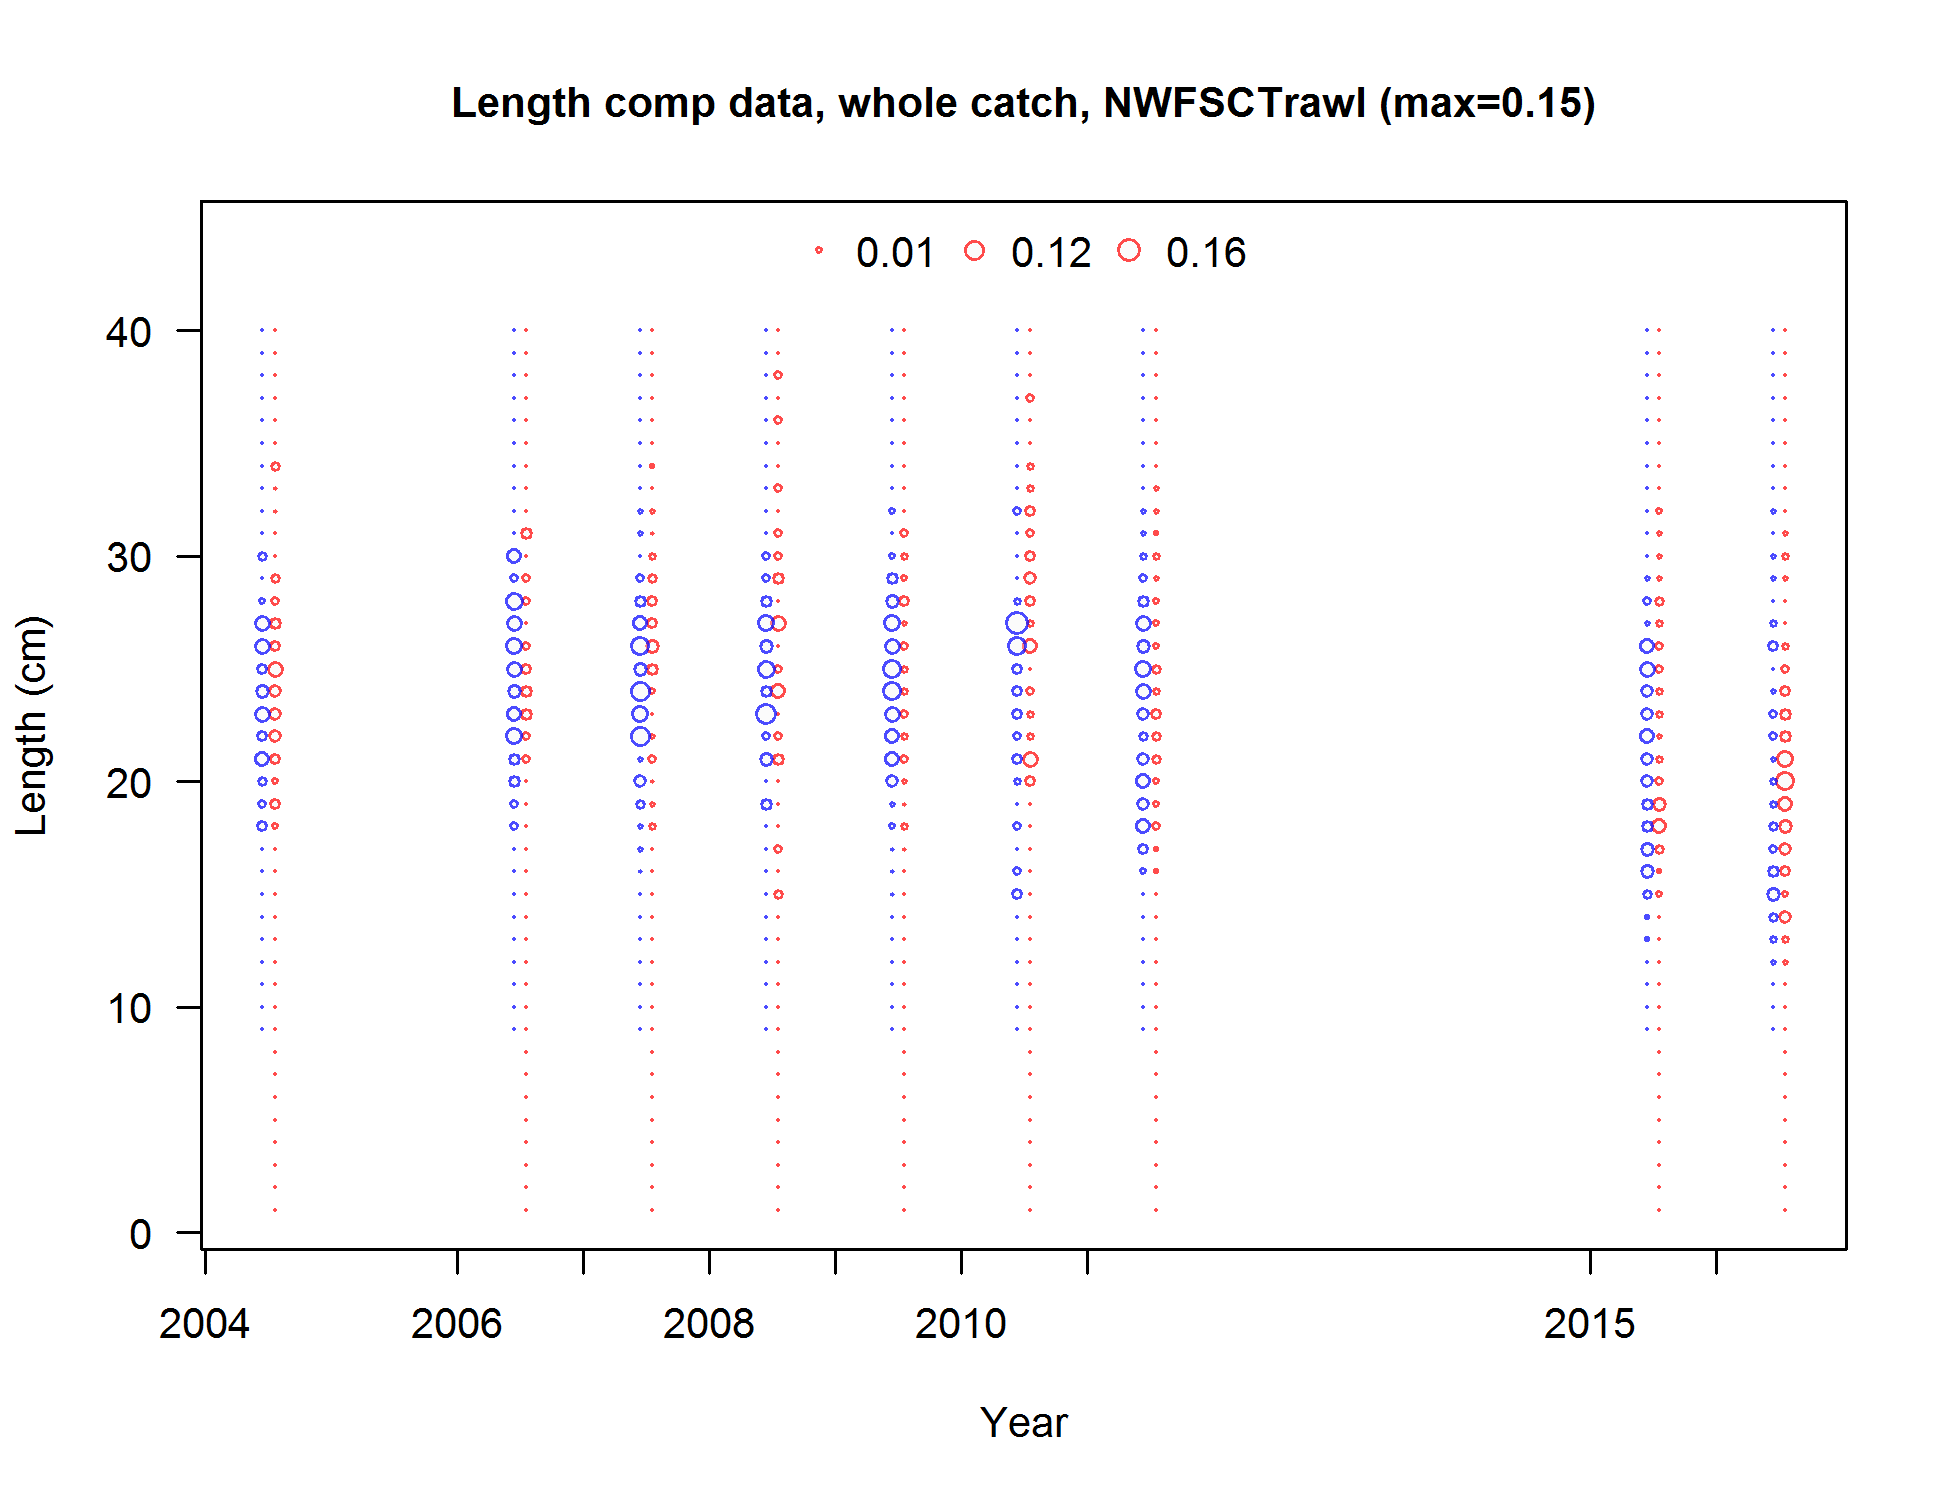
\includegraphics{r4ss/plots_mod1/comp_lendat_bubflt8mkt0.png}

\endcol
\endcols

\end{frame}

\subsection{Maturity and Fecundity}\label{maturity-and-fecundity}

\begin{itemize}
\item[$\circ$] Only information on maturity from Love et al. (1987)
\item[$\circ$] Found over 50\% of females were mature by 18 cm TL, or two years of age. 
\item[$\circ$] All fish were mature by 22 cm TL
\item[$\circ$] No information available on fecundity of California scorpionfish
\end{itemize}

\subsection{Weight-at-length}\label{weight-at-length}

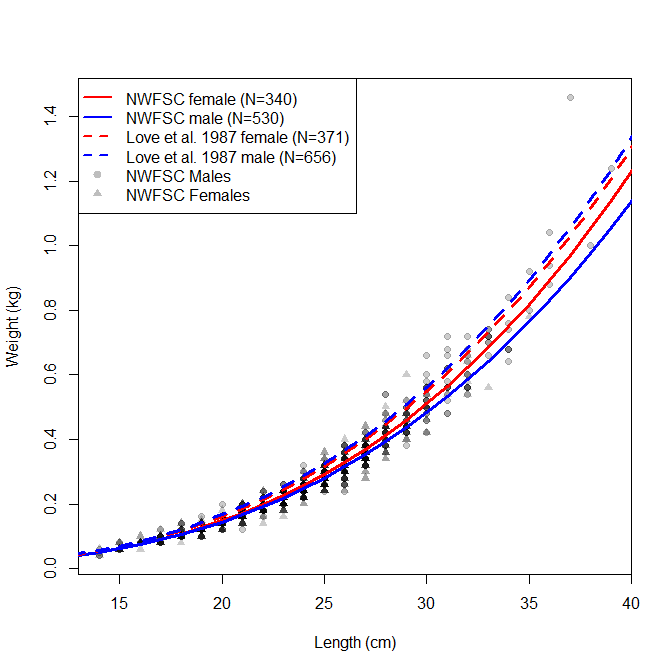
\includegraphics{Figures/Length_weight.png}

\subsection{Natural mortality}\label{natural-mortality}

\begin{itemize}
\item[$\circ$] Prior based on maximum age of 21
\item[$\circ$] Lognormal distribution with a median of 0.2715
\item[$\circ$] Base model fixes female natural mortality ($M$)
\item[$\circ$] Male $M$ estiamted as offset from female $M$
\item[$\circ$] Sensitivities explore estimating $M$
\end{itemize}

\subsection{Steepness: Density-Dependent Recruitment
Compensation}\label{steepness-density-dependent-recruitment-compensation}

\begin{itemize}
\item[$\circ$] Predictive distribution for Pacific rockfish meta-analysis
\item[$\circ$] Preior mediant in 2017 for steepness ($h$) = 0.718
\end{itemize}

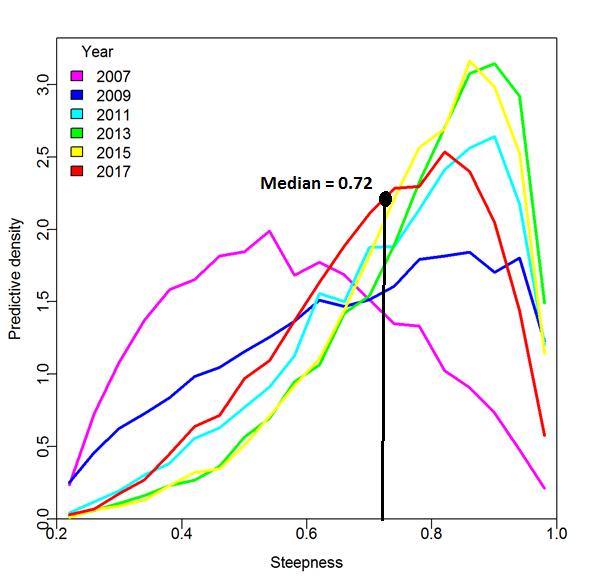
\includegraphics{Figures/h_prior.png}

\section{Removals}\label{removals}

\subsection{Total Removals}\label{total-removals}

\centering
\includegraphics{California_scorpionfish_2017_files/figure-latex/unnamed-chunk-16-1.pdf}

\subsection{Total Removals}\label{total-removals-1}

\includegraphics{California_scorpionfish_2017_files/figure-latex/unnamed-chunk-17-1.pdf}

\subsection{Total Removals}\label{total-removals-2}

\includegraphics{California_scorpionfish_2017_files/figure-latex/unnamed-chunk-18-1.pdf}

\subsection{Commercial Landings by
Fleet}\label{commercial-landings-by-fleet}

\subsection{Recreational Landings by
Fleet}\label{recreational-landings-by-fleet}

\section{Index Data}\label{index-data}

\subsection{Summary of Data Sources}\label{summary-of-data-sources}

\begin{itemize}
\tightlist
\item
  All of the methods used to standardize indices have been endorsed by
  the SSC
\end{itemize}

\begin{table}[ht]
\centering
\scalebox{0.7}{
\begin{tabular}{p{2.5in}p{0.8in}p{.4in}p{2in}}
  \hline
Name & Years & Fishery ind. & Method \\ 
  \hline
Recreational PR dockside CPUE & 2004-2016 & No & delta-GLM (bin-lognormal) \\ 
  CPFV logbook CPUE & 1980-2016 & No & negative binomial \\ 
  Onboard observer discard catch CPUE & 2002-2016 & No & delta-GLM (bin-lognormal) \\ 
  Sanitation district CPUE & 1970-2016 & Yes & delta-GLM (bin-lognormal) \\ 
  NWFSC trawl survey CPUE & 2003-2016 & Yes & VAST \\ 
  CSUN/VRG Gillnet survey CPUE & 1995-2008 & Yes & delta-GLM (bin-lognormal) \\ 
  Southern Califrnia Bight trawl survey CPUE & '94, '98, '03, '08, '13 & Yes & delta-GLM (bin-lognormal) \\ 
  Onboard observer retained catch CPUE & 2002-2016 & No & delta-GLM (bin-lognormal) \\ 
   \hline
\end{tabular}
}
\end{table}

\subsection{Recreational Private Boat
Index}\label{recreational-private-boat-index}

\subsection{Recreational Party/Charter Boat Index
(Logbook)}\label{recreational-partycharter-boat-index-logbook}

\subsection{Recreational Dead Discard
Index}\label{recreational-dead-discard-index}

\subsection{Recreational Party/Charter Retained Catch
Index}\label{recreational-partycharter-retained-catch-index}

\subsection{Sanitation Districts Survey
Index}\label{sanitation-districts-survey-index}

\begin{table}[ht]
\centering
\scalebox{0.9}{
\begin{tabular}{lrrrrr}
  \hline
Program & 0-24 m & 25-49 m & 50-74m & 100+ m & Total \\ 
  \hline
City of Los Angeles & 120 &   0 & 1372 &   0 & 1492 \\ 
  Los Angeles County & 687 &   0 & 5879 & 450 & 7016 \\ 
  Orange County & 161 & 669 & 2157 &  48 & 3035 \\ 
  City of San Diego &   0 & 404 & 333 & 829 & 1566 \\ 
   \hline
\end{tabular}
}
\end{table}

\subsection{Sanitation Districts Survey
Index}\label{sanitation-districts-survey-index-1}

\subsection{Sanitation Districts Survey
Index}\label{sanitation-districts-survey-index-2}

\subsection{NWFSC Trawl Survey Index}\label{nwfsc-trawl-survey-index}

\subsection{Gillnet Survey Index}\label{gillnet-survey-index}

\subsection{Southern California Bight Trawl Survey
Index}\label{southern-california-bight-trawl-survey-index}

\section{Composition Data}\label{composition-data}

\subsection{Dat1}\label{dat1}

\subsection{Summary of Data used in the 2017
Assessment}\label{summary-of-data-used-in-the-2017-assessment}

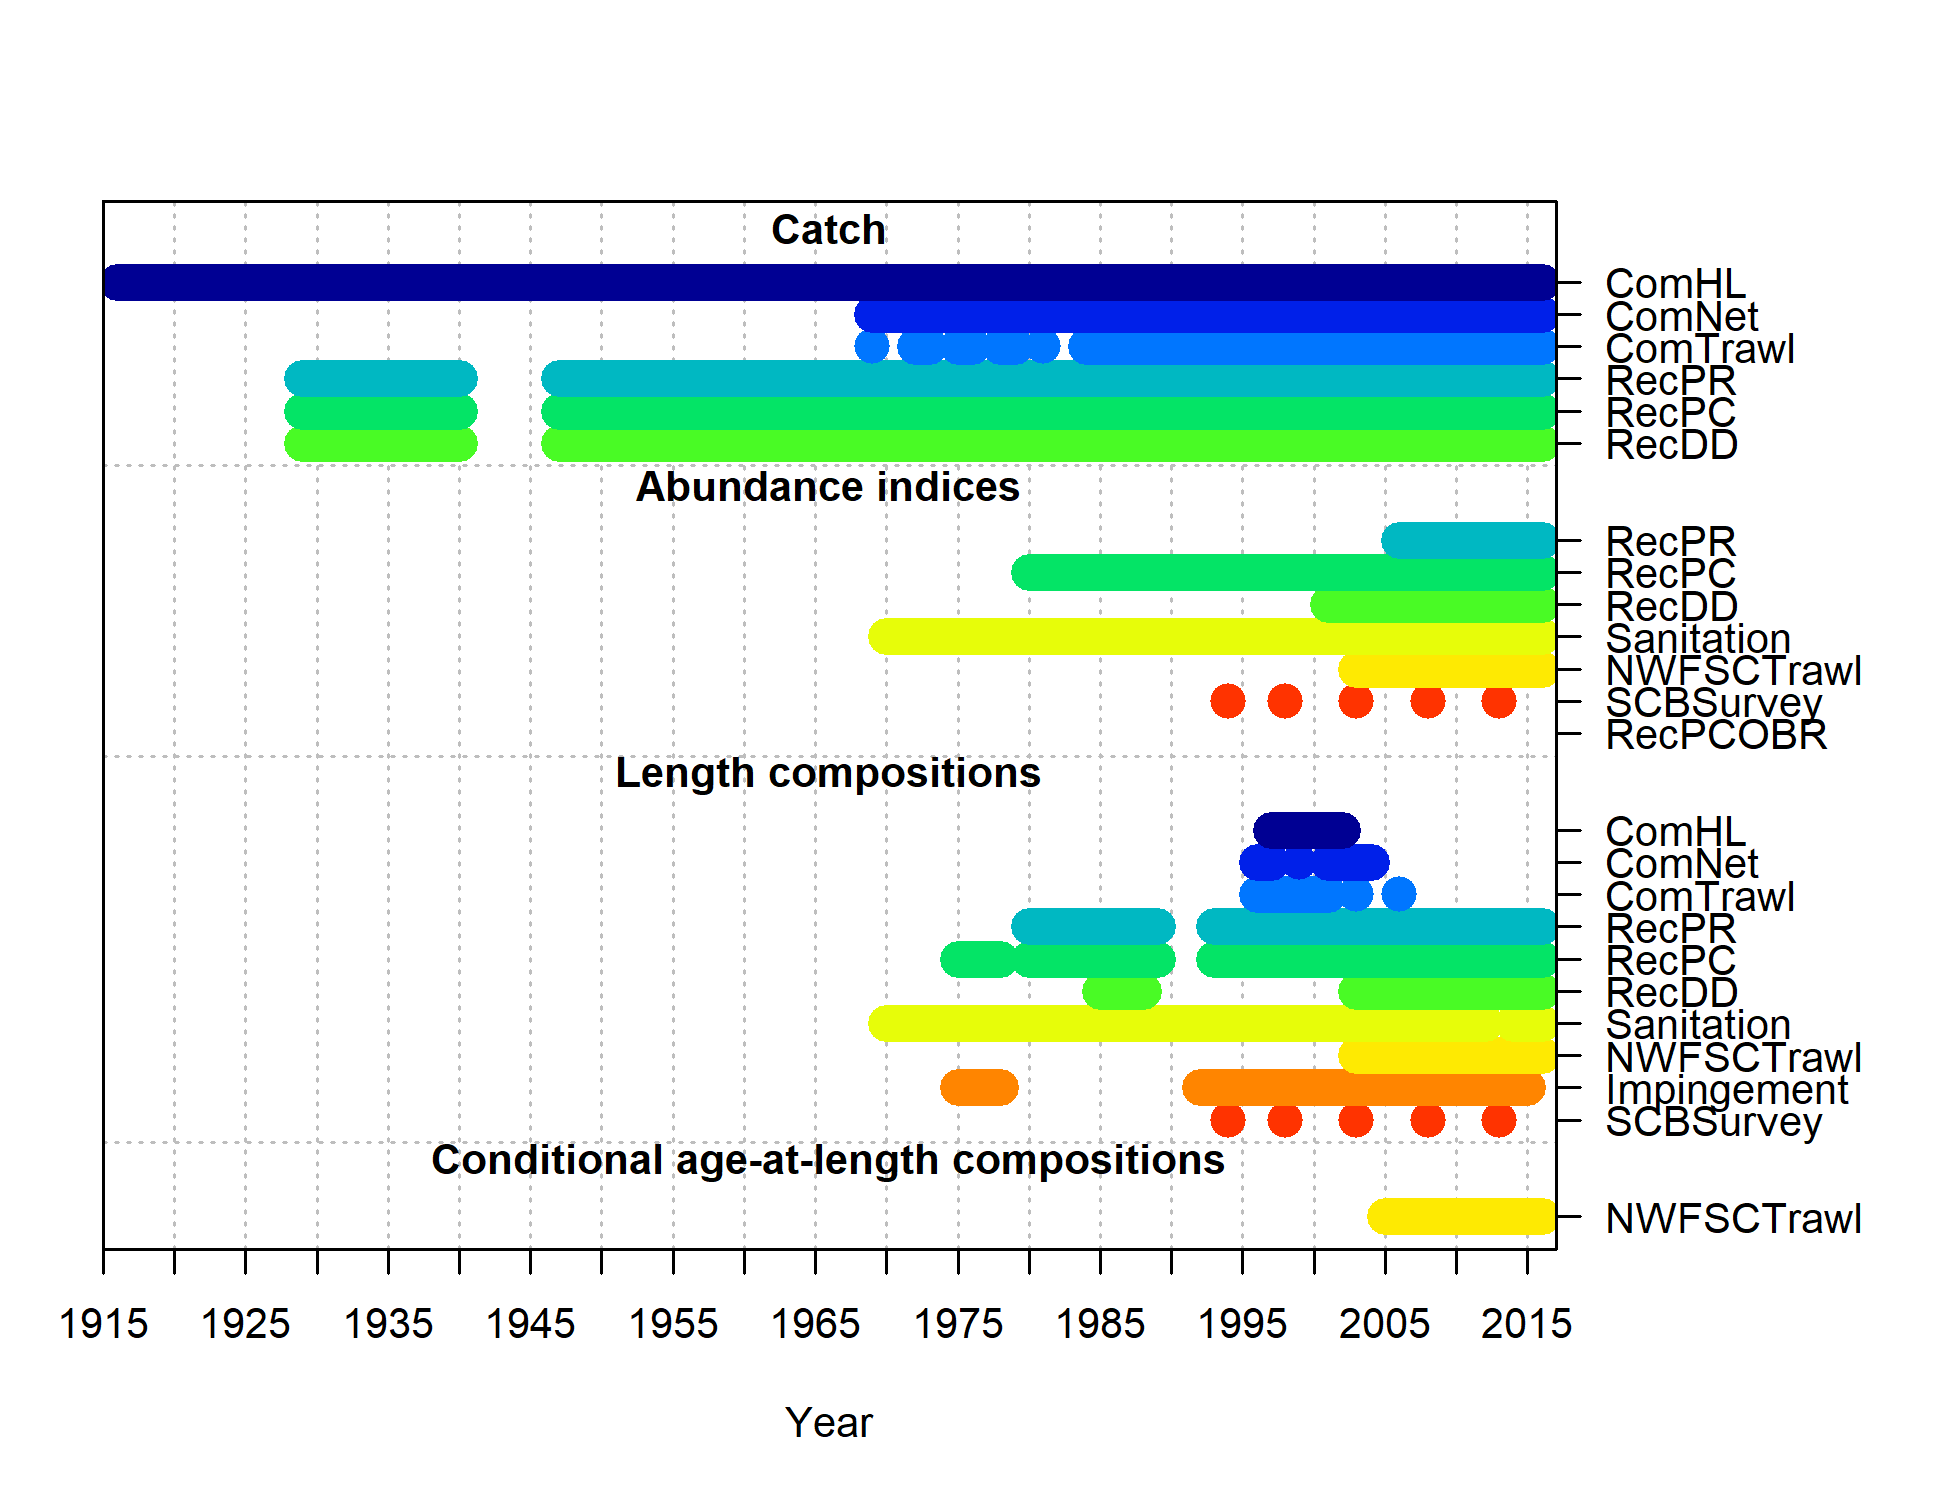
\includegraphics{r4ss/plots_mod1/data_plot.png}

\section{2017 assessment}\label{assessment}

\section{Uncertainty and
Sensitivities}\label{uncertainty-and-sensitivities}

\section{Additional slides}\label{additional-slides}

\FloatBarrier
\newpage

\section*{Appendix A. Detailed fits to length composition
data}\label{appendix-a.-detailed-fits-to-length-composition-data}
\addcontentsline{toc}{section}{Appendix A. Detailed fits to length
composition data}

\renewcommand{\thepage}{A-\arabic{page}}
\renewcommand{\thefigure}{A\arabic{figure}}

\setcounter{page}{1}

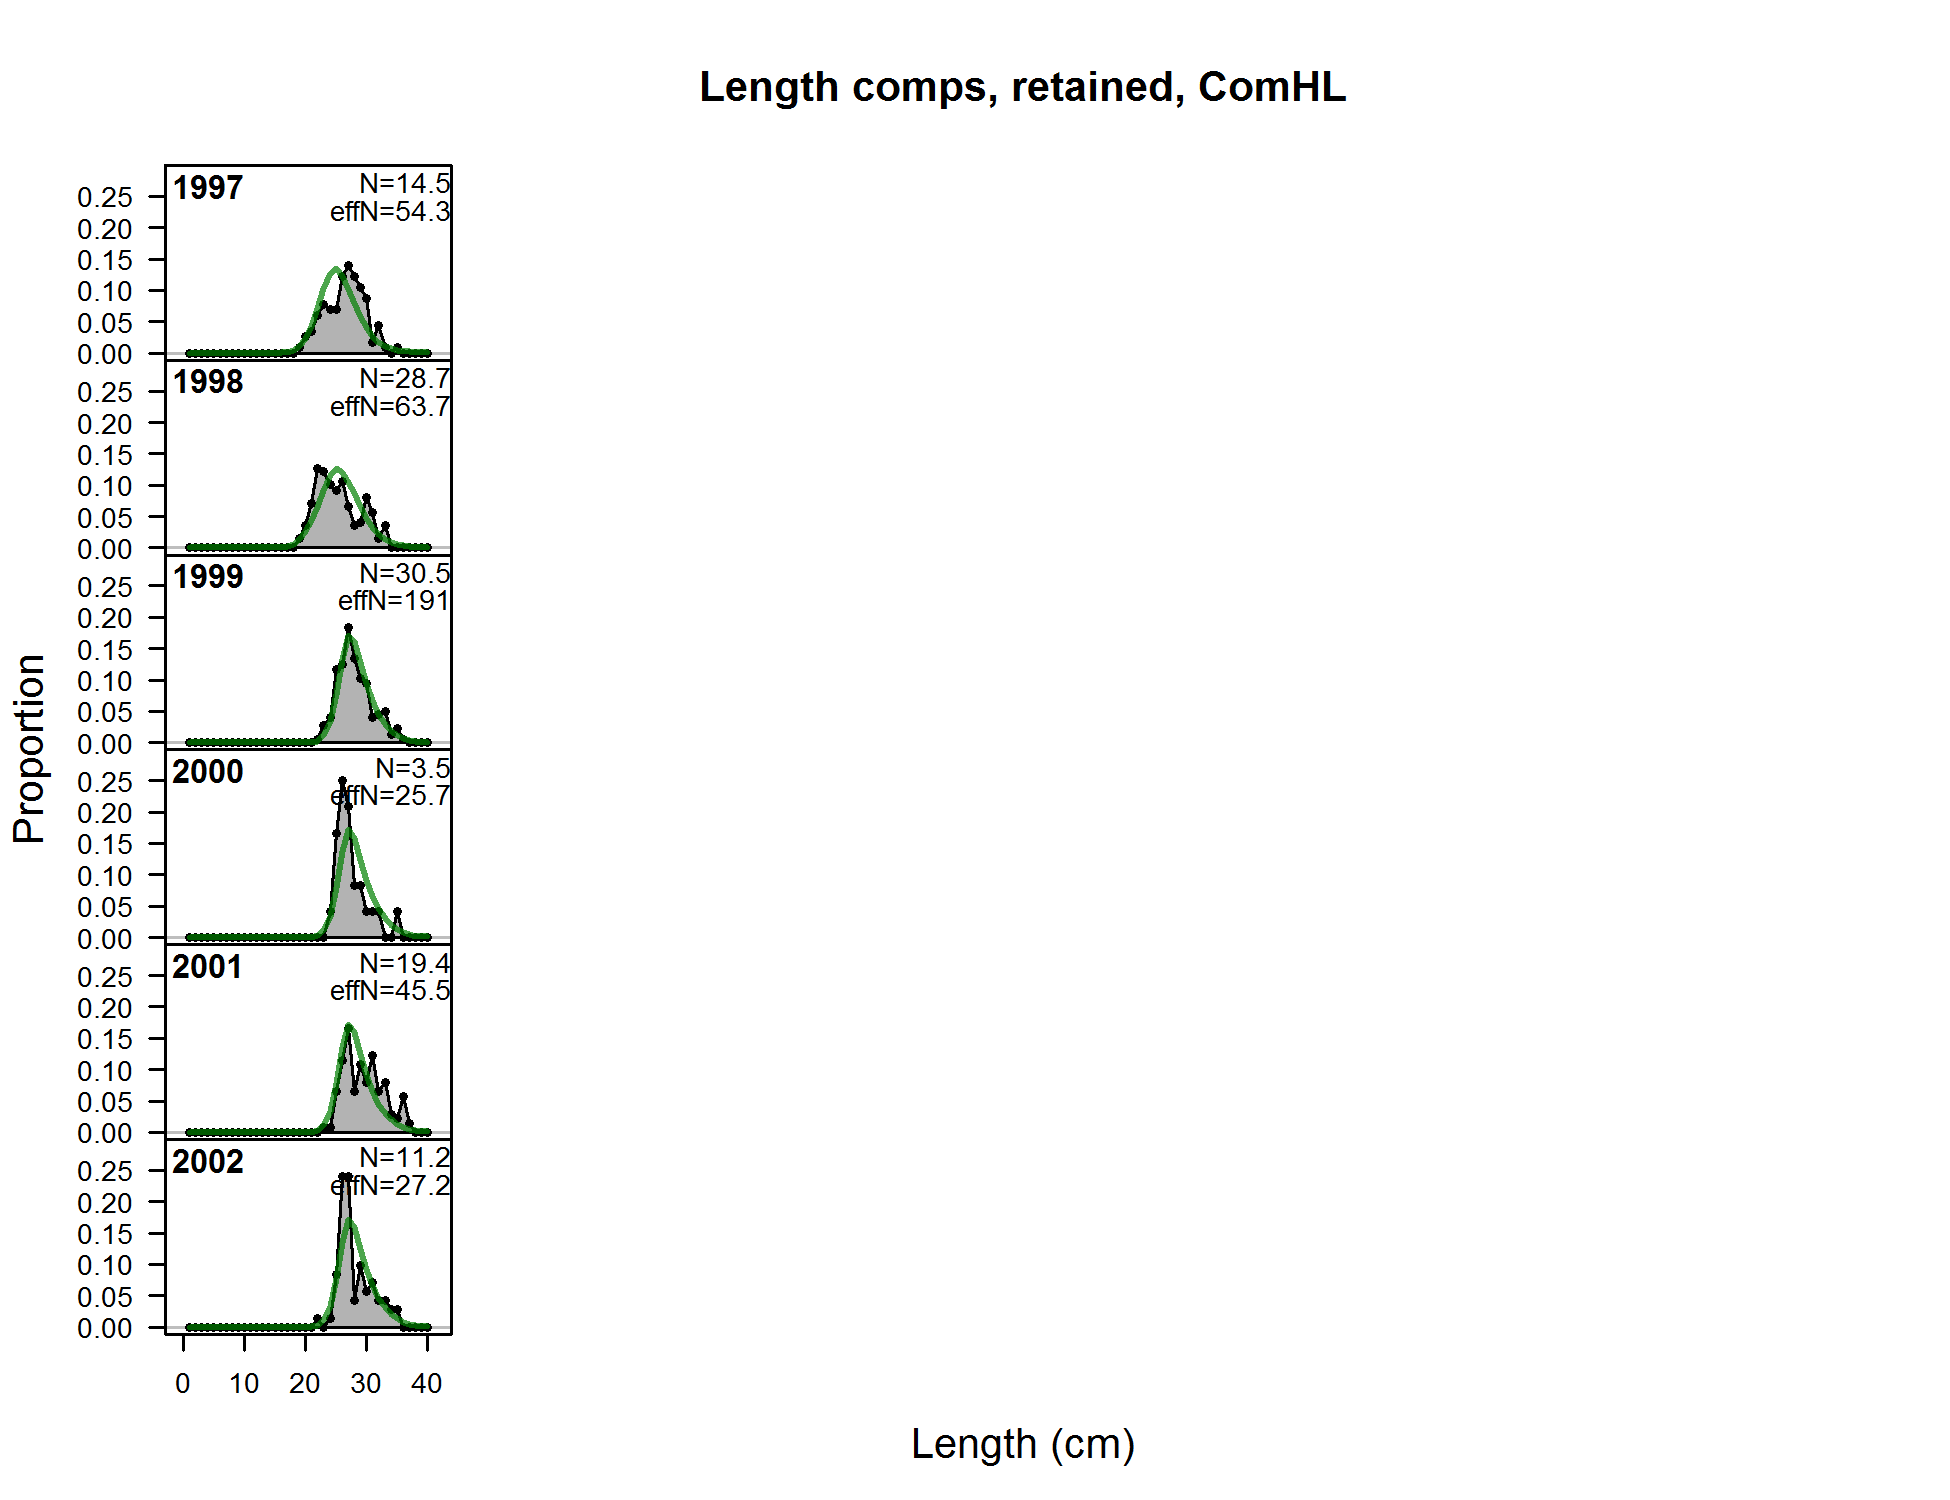
\includegraphics{./r4ss/plots_mod1/comp_lenfit_flt1mkt2.png}

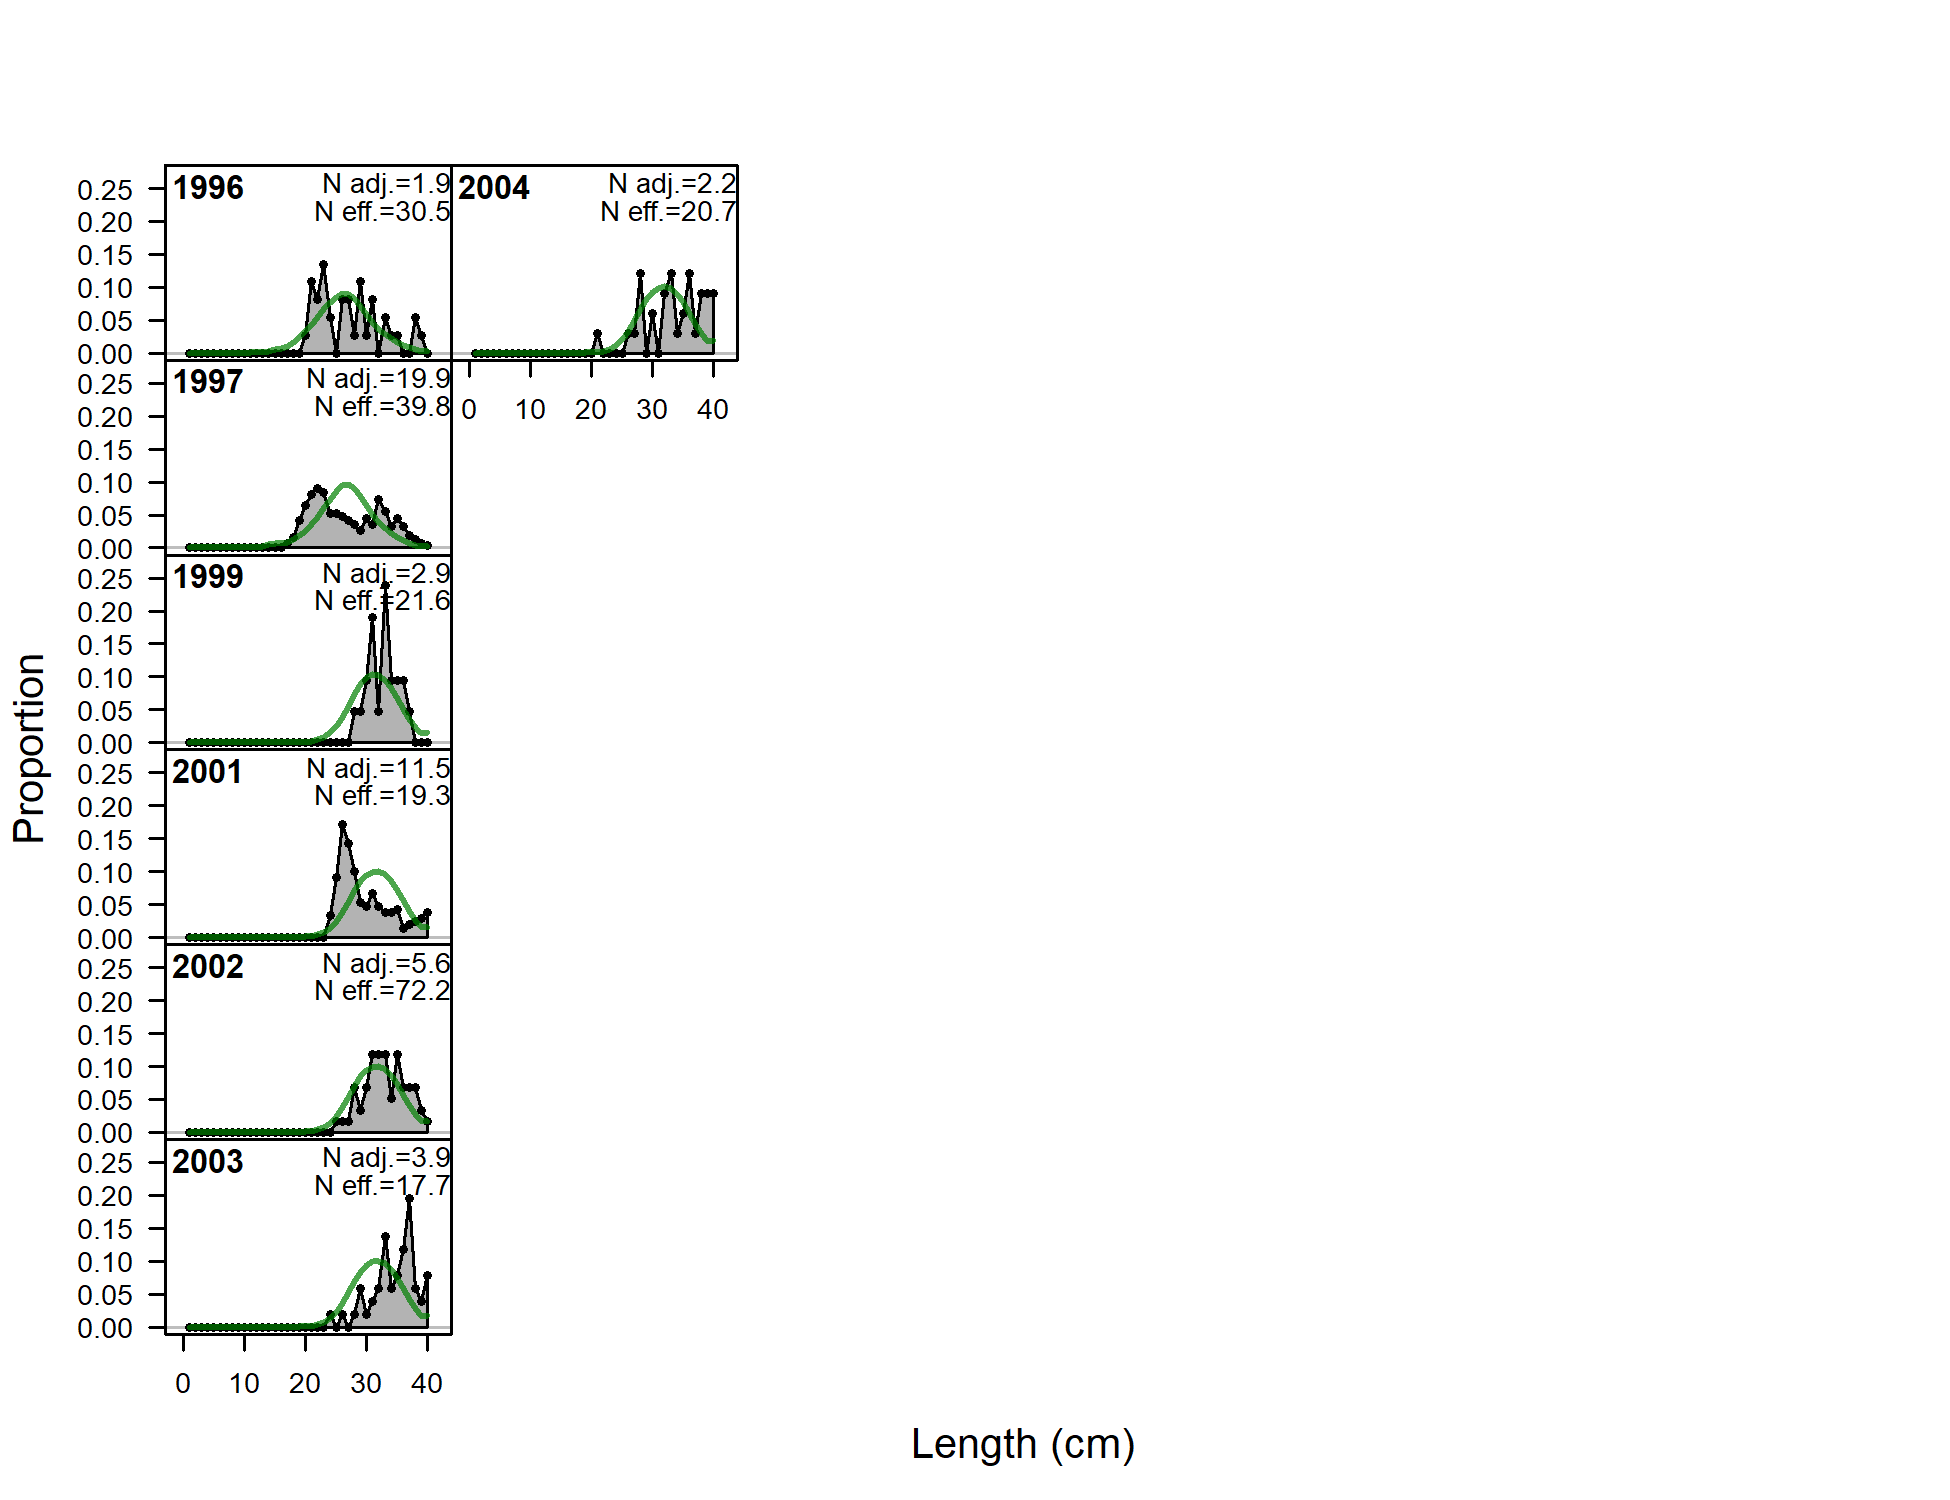
\includegraphics{./r4ss/plots_mod1/comp_lenfit_flt2mkt2.png}

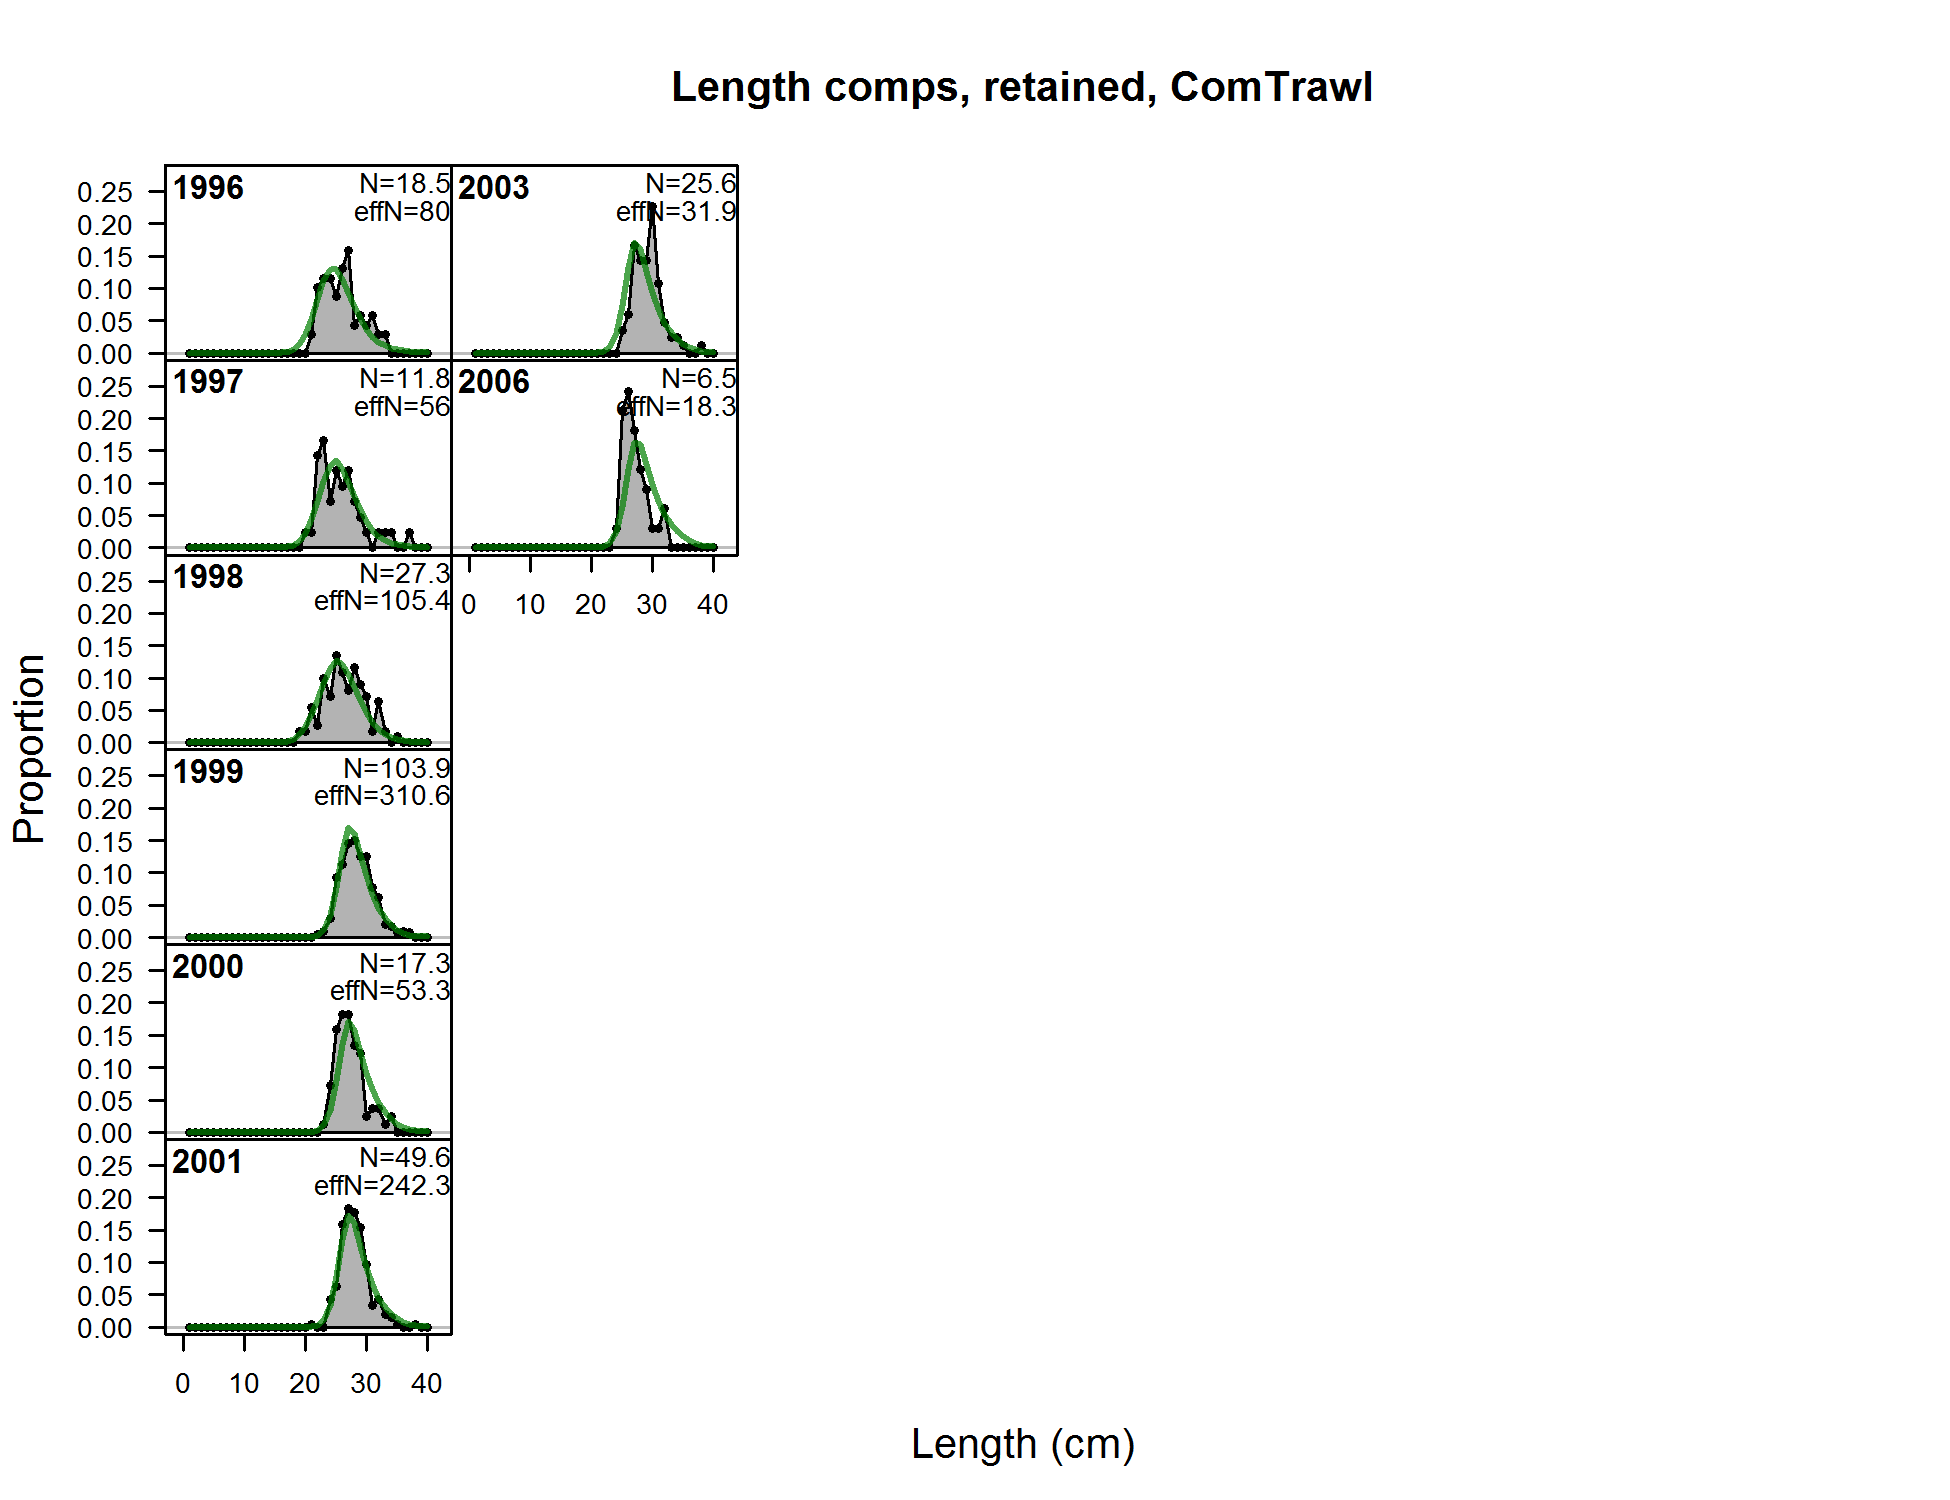
\includegraphics{./r4ss/plots_mod1/comp_lenfit_flt3mkt2.png}

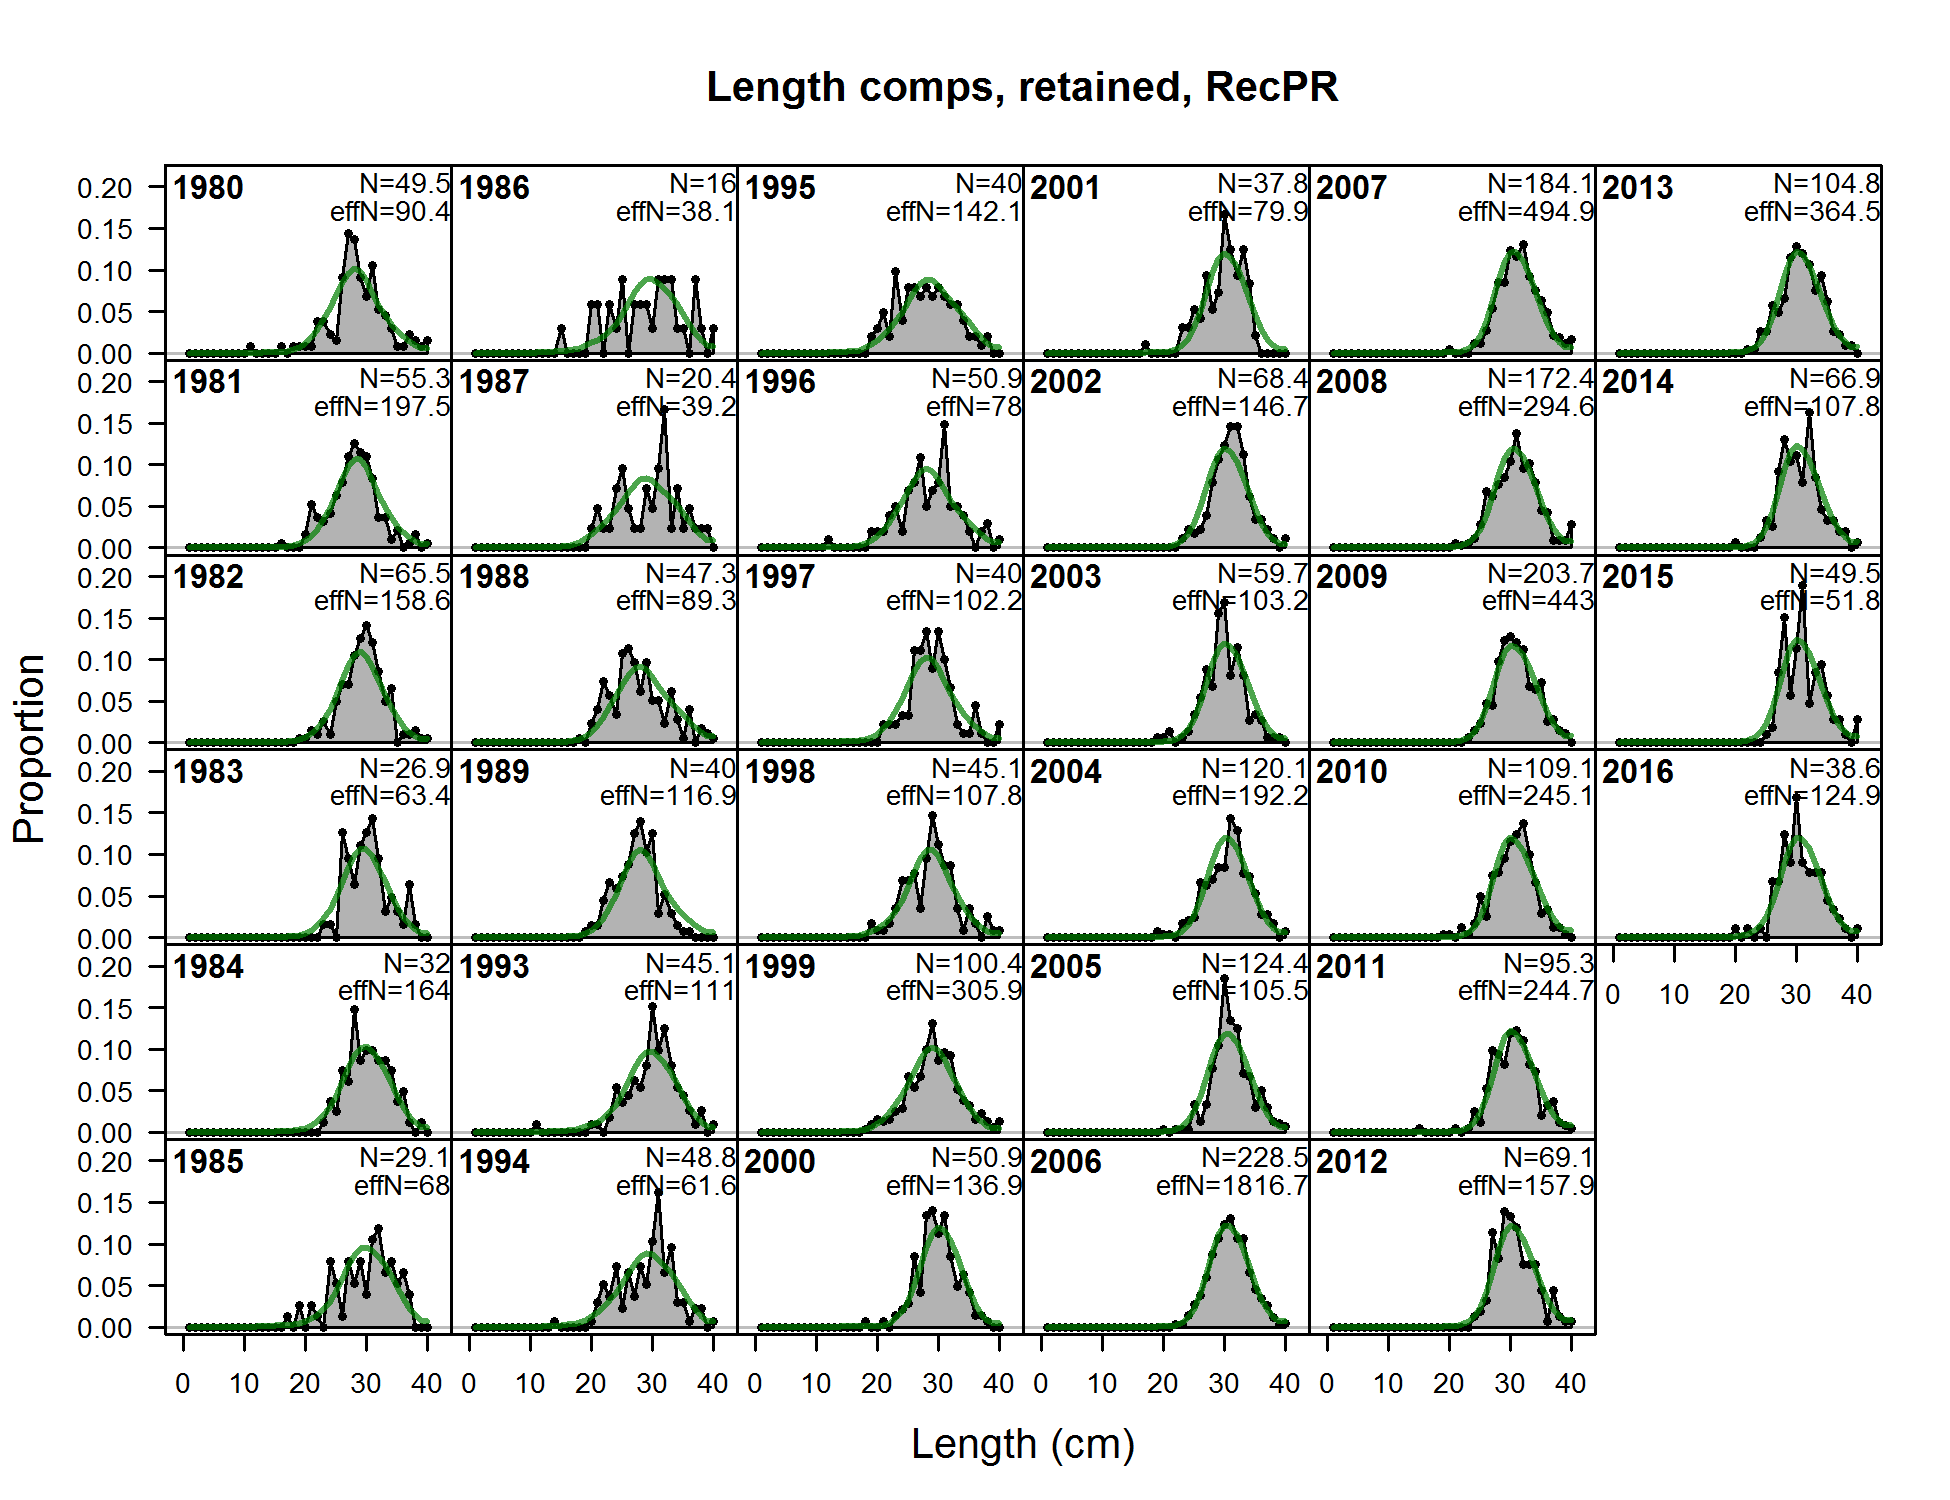
\includegraphics{./r4ss/plots_mod1/comp_lenfit_flt4mkt2.png}

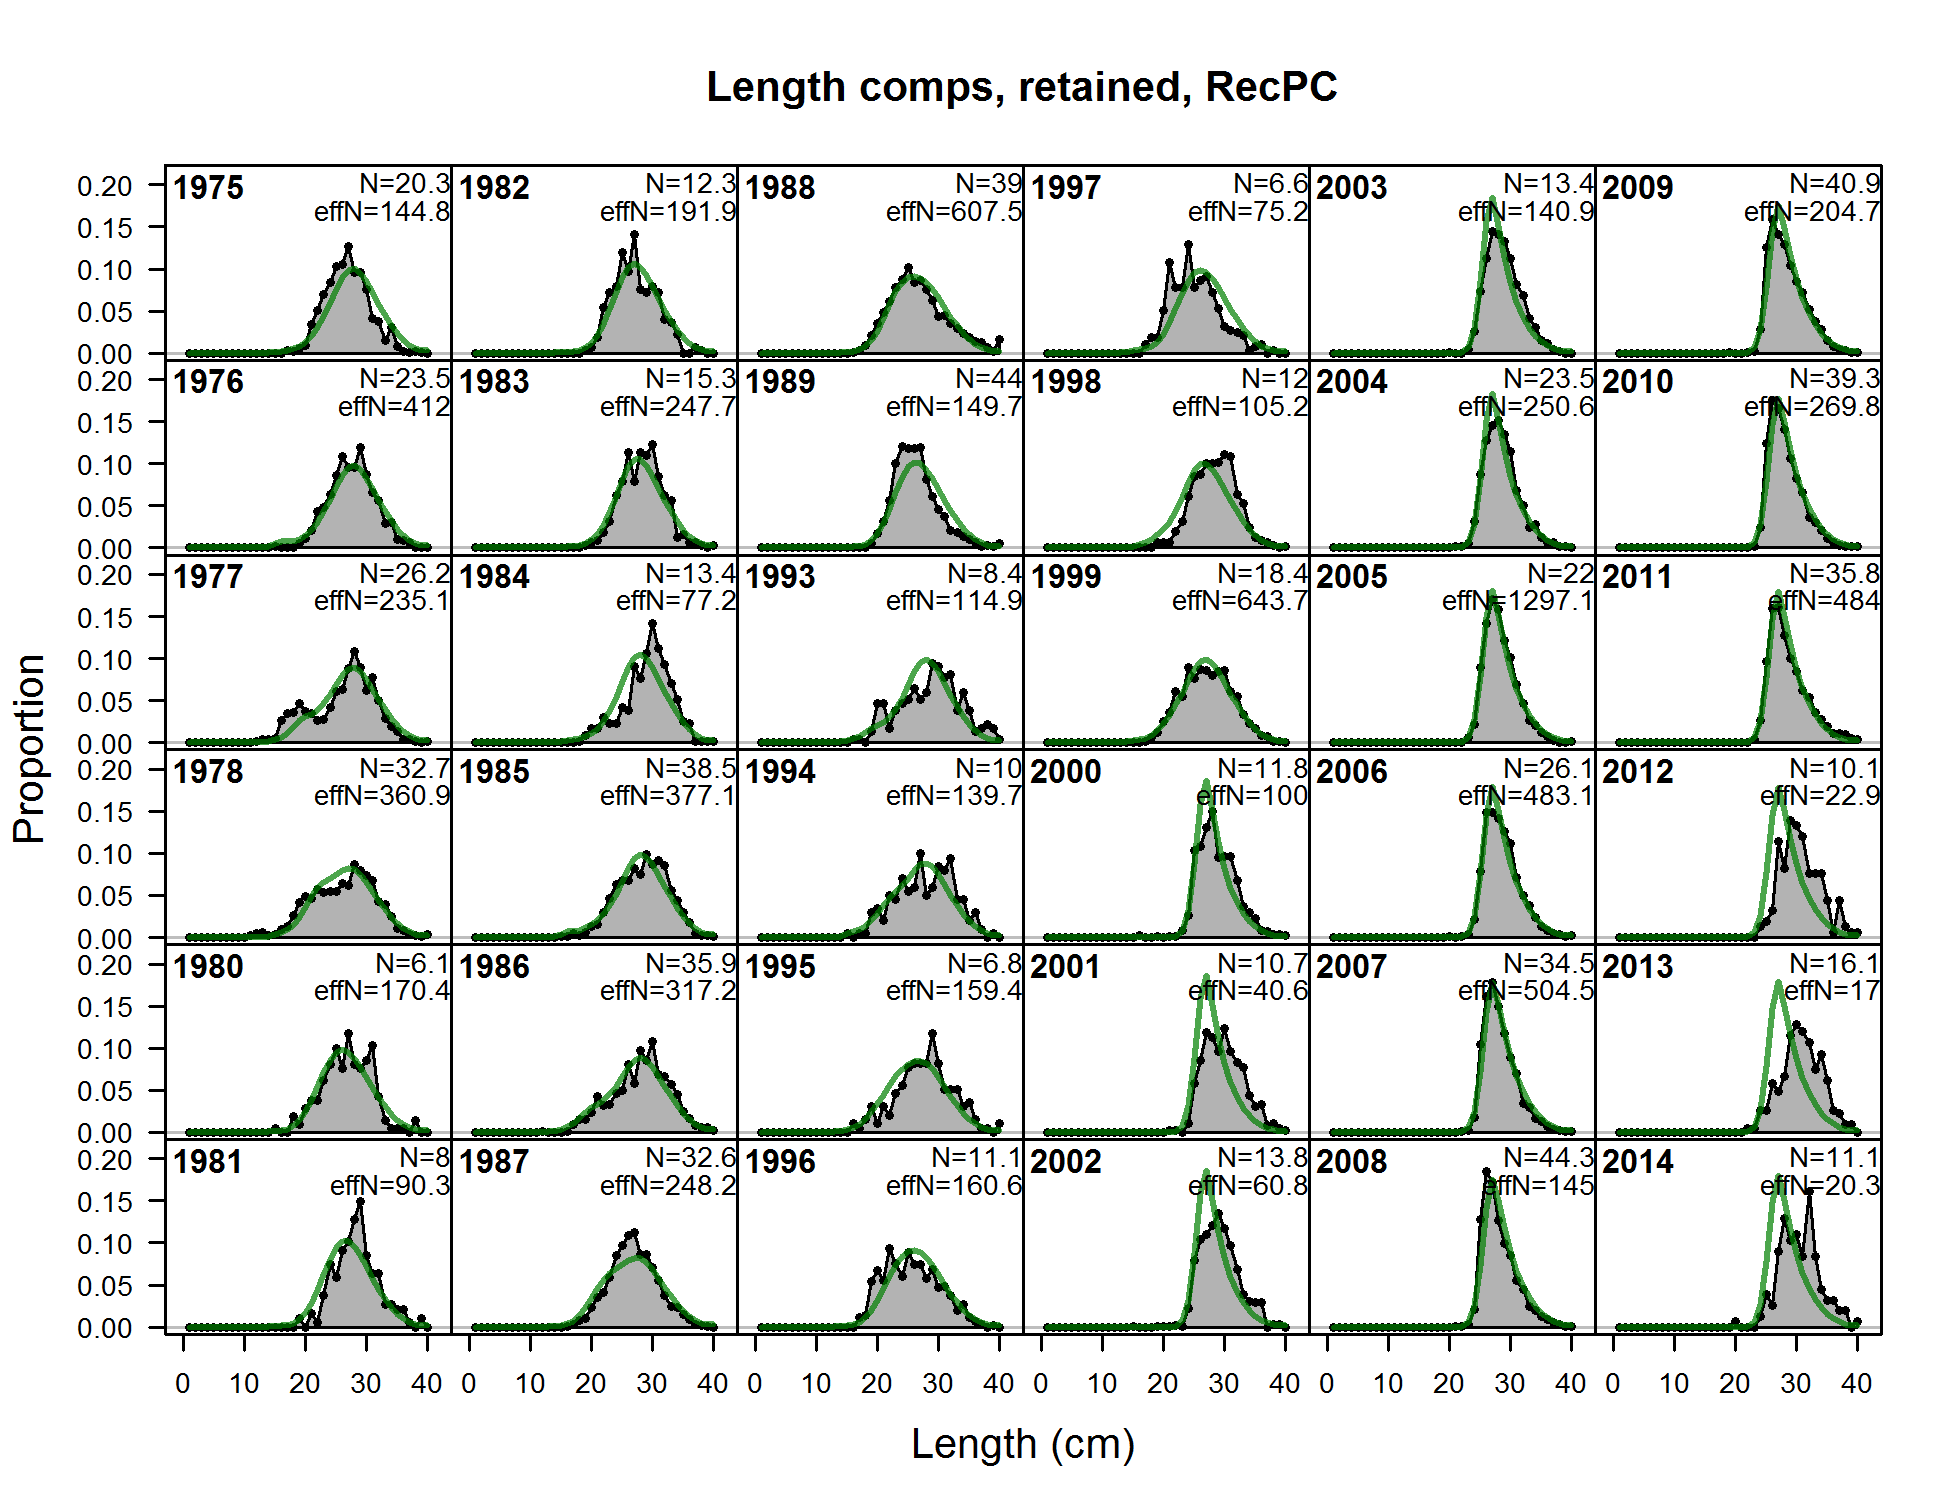
\includegraphics{./r4ss/plots_mod1/comp_lenfit_flt5mkt2_page1.png}

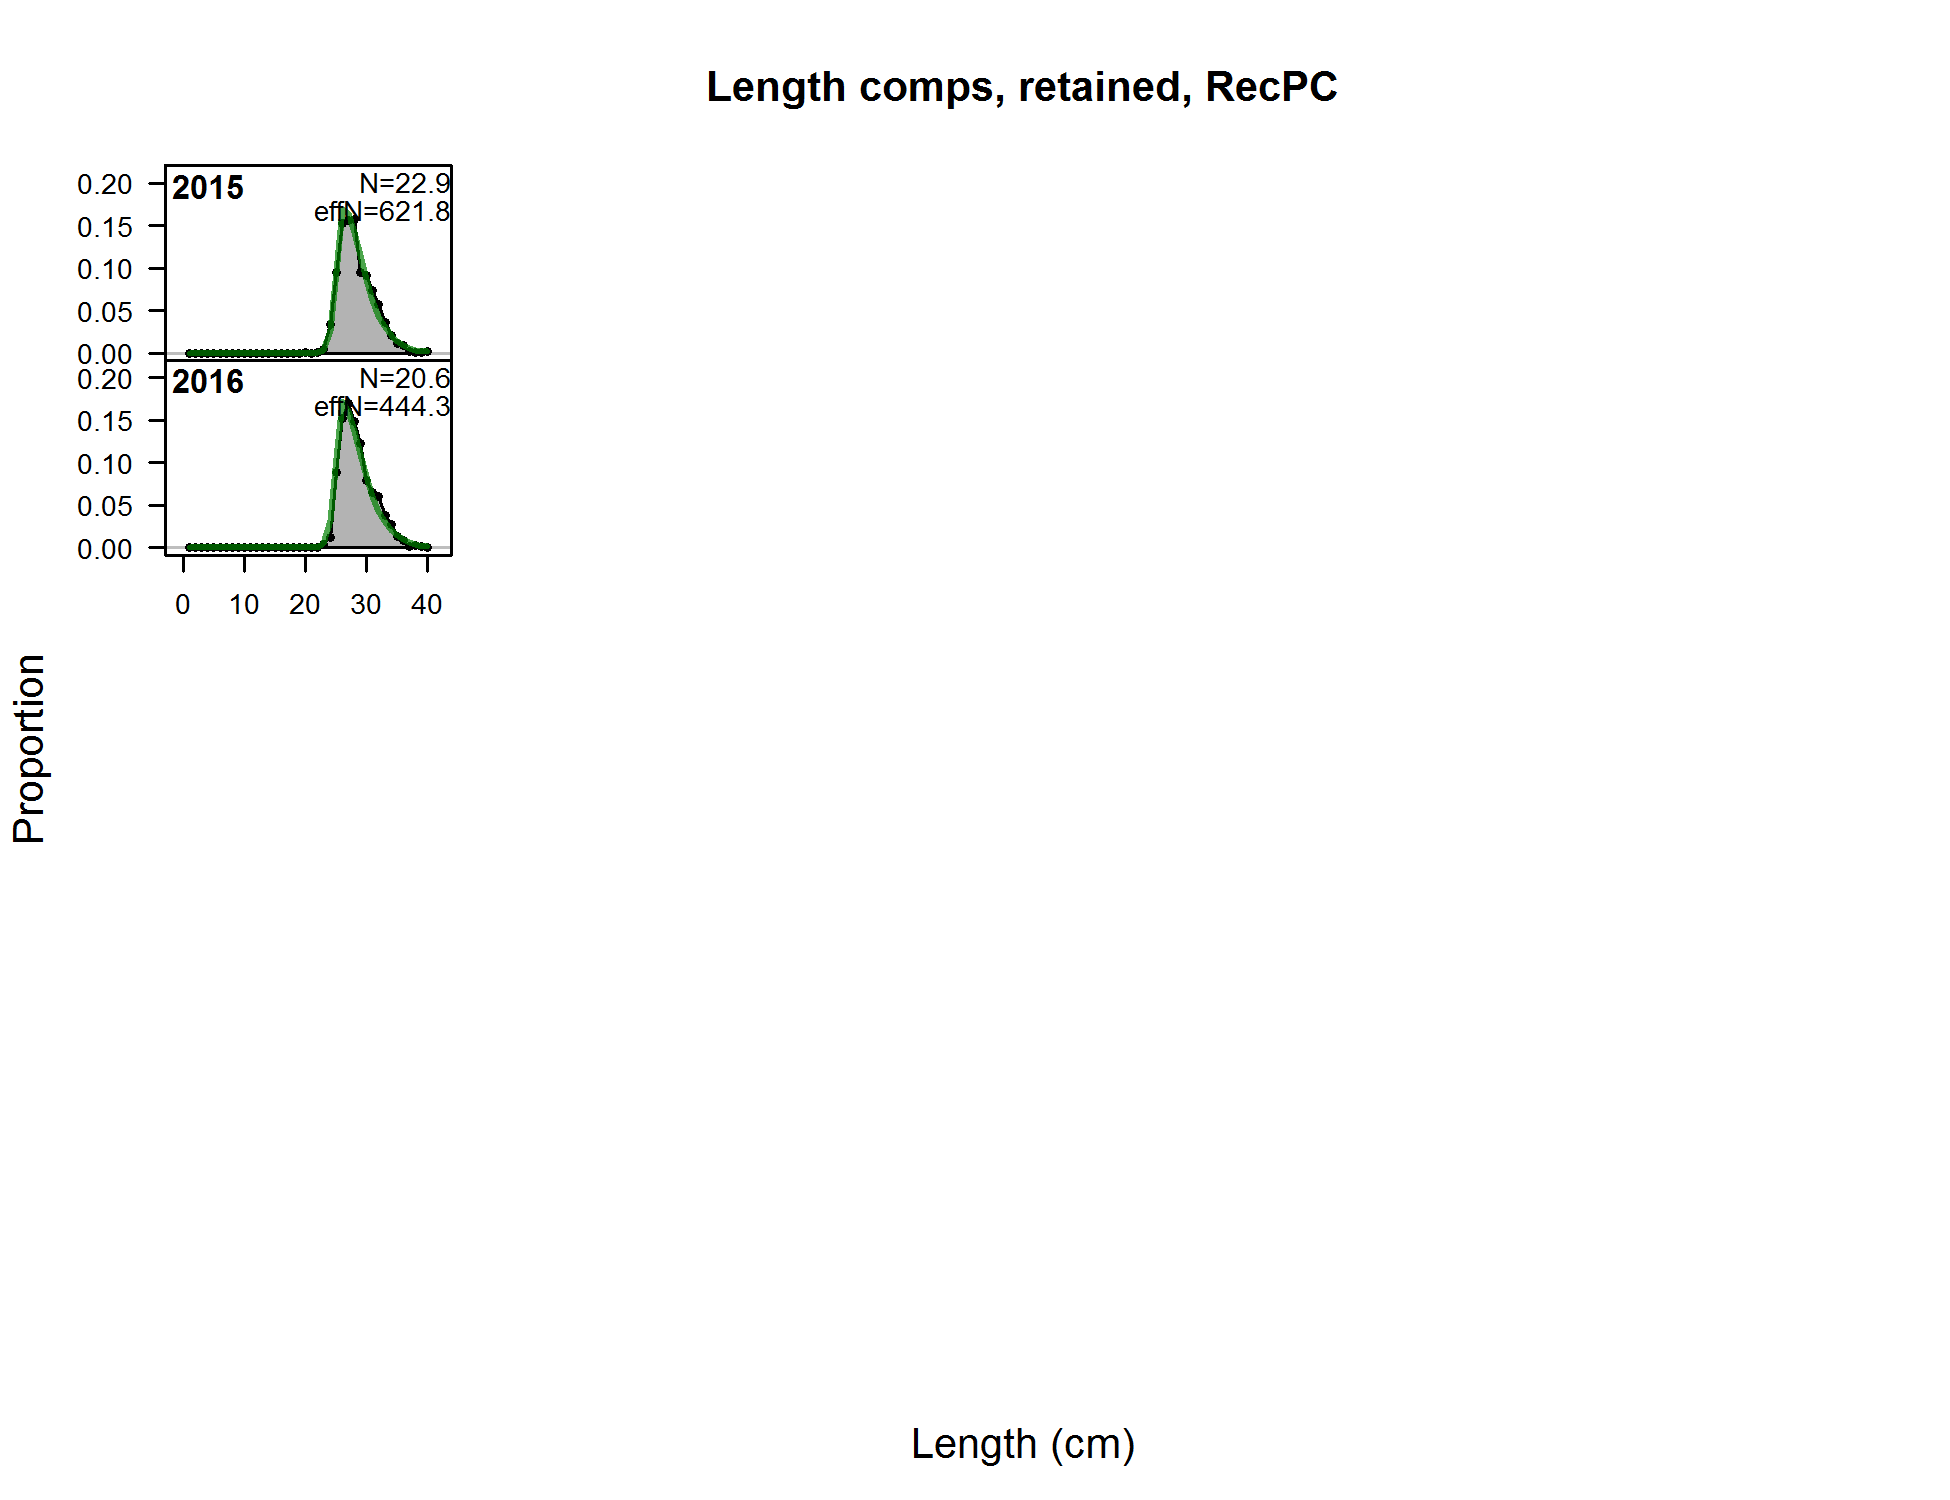
\includegraphics{./r4ss/plots_mod1/comp_lenfit_flt5mkt2_page2.png}

\begin{center} 

              Figure continued from previous page 

             \end{center}

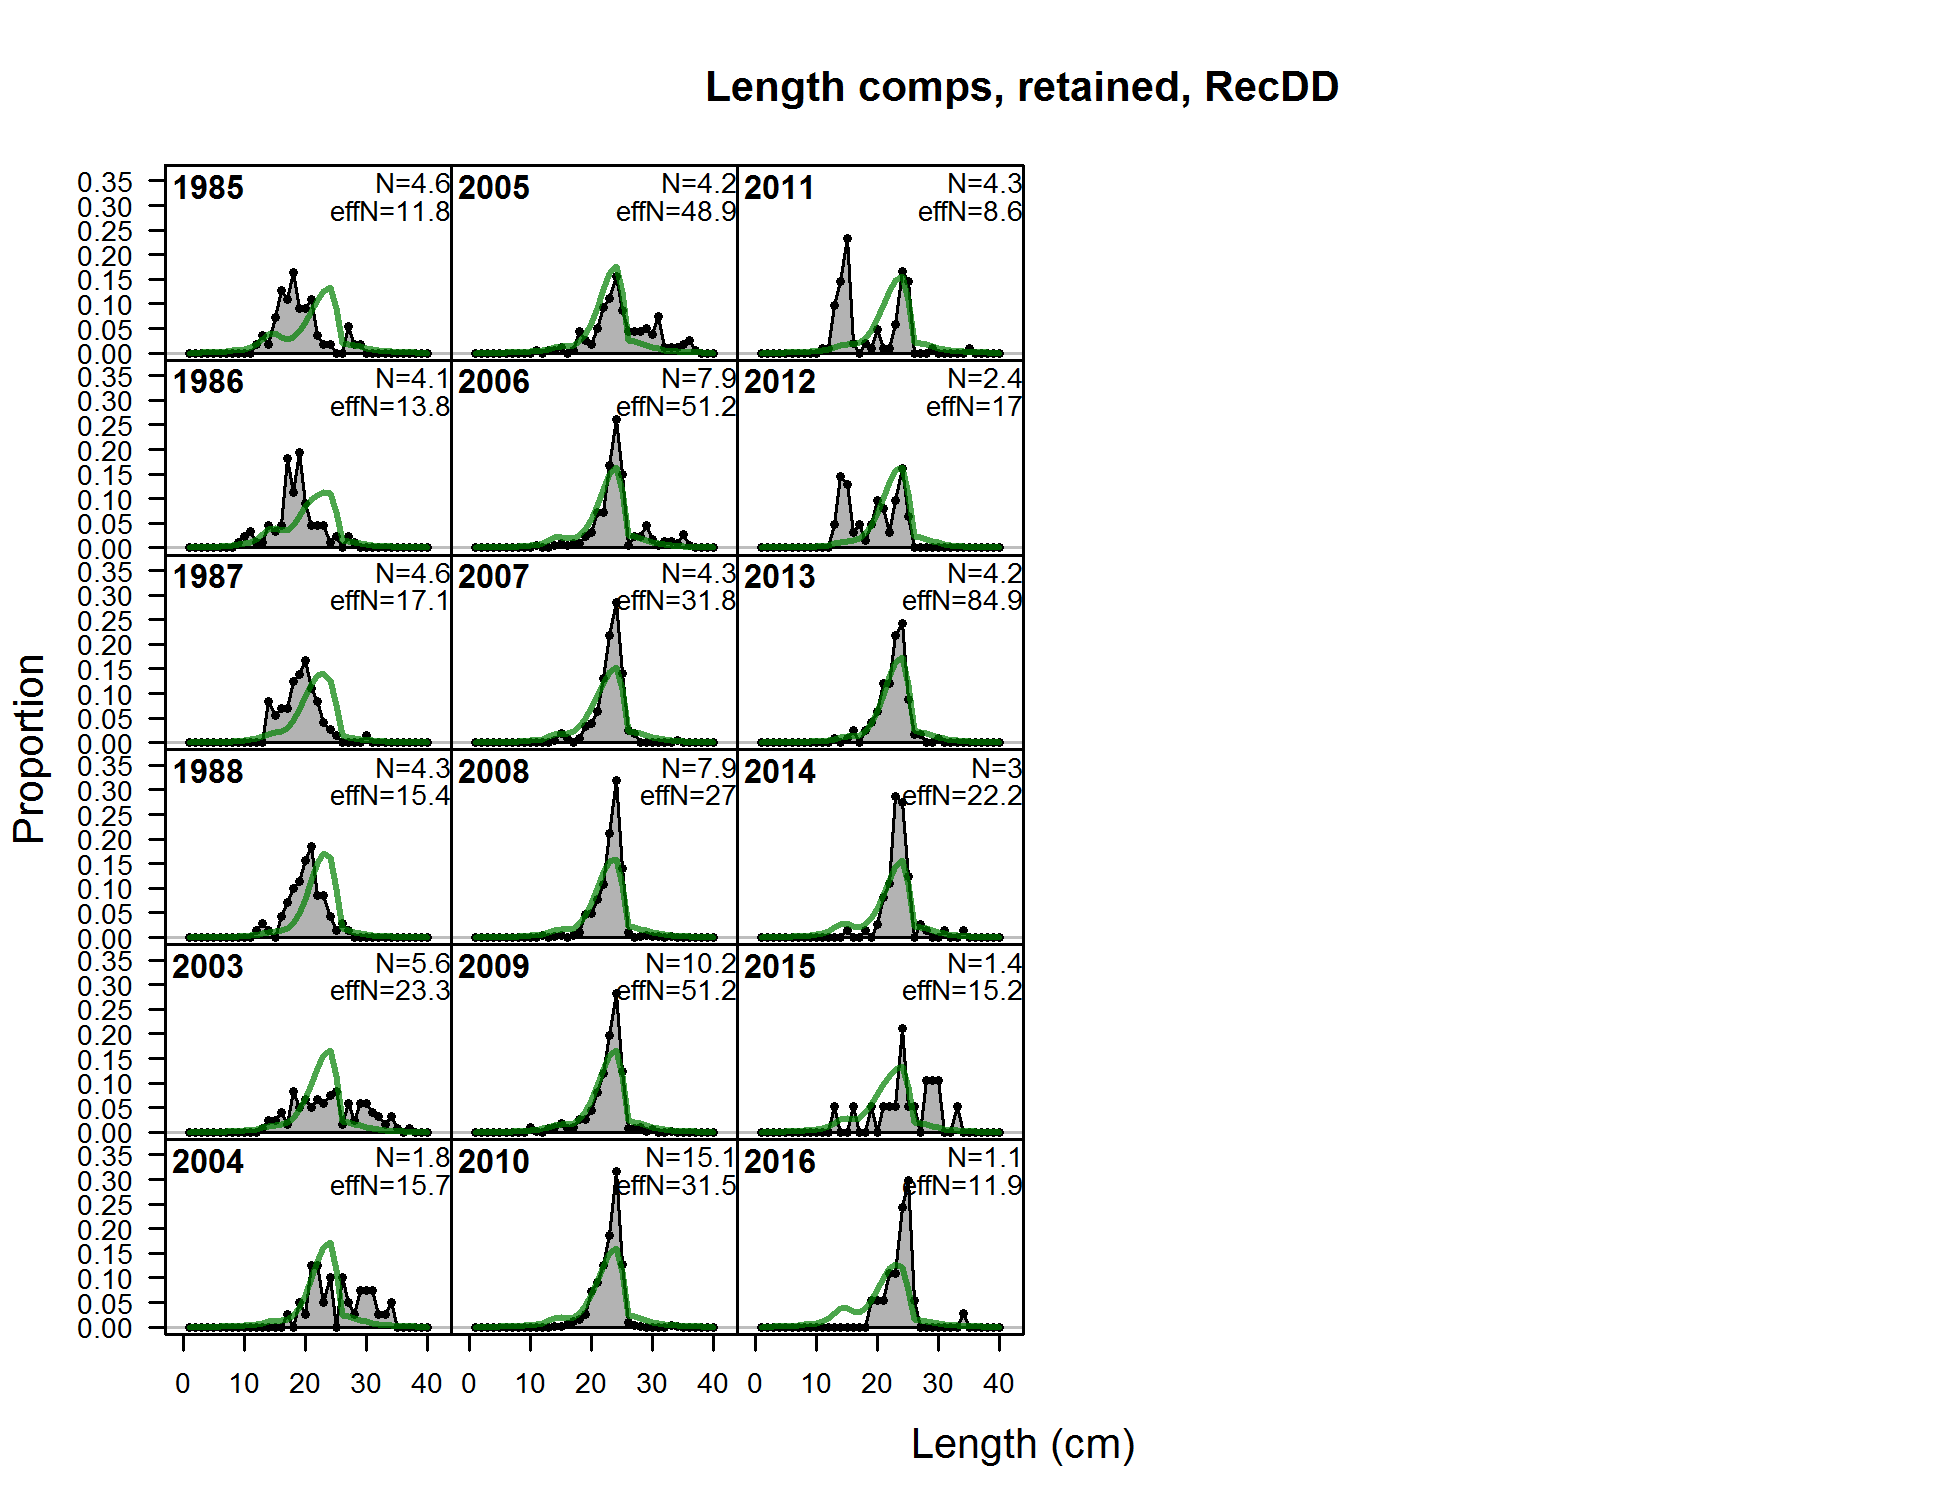
\includegraphics{./r4ss/plots_mod1/comp_lenfit_flt6mkt2.png}

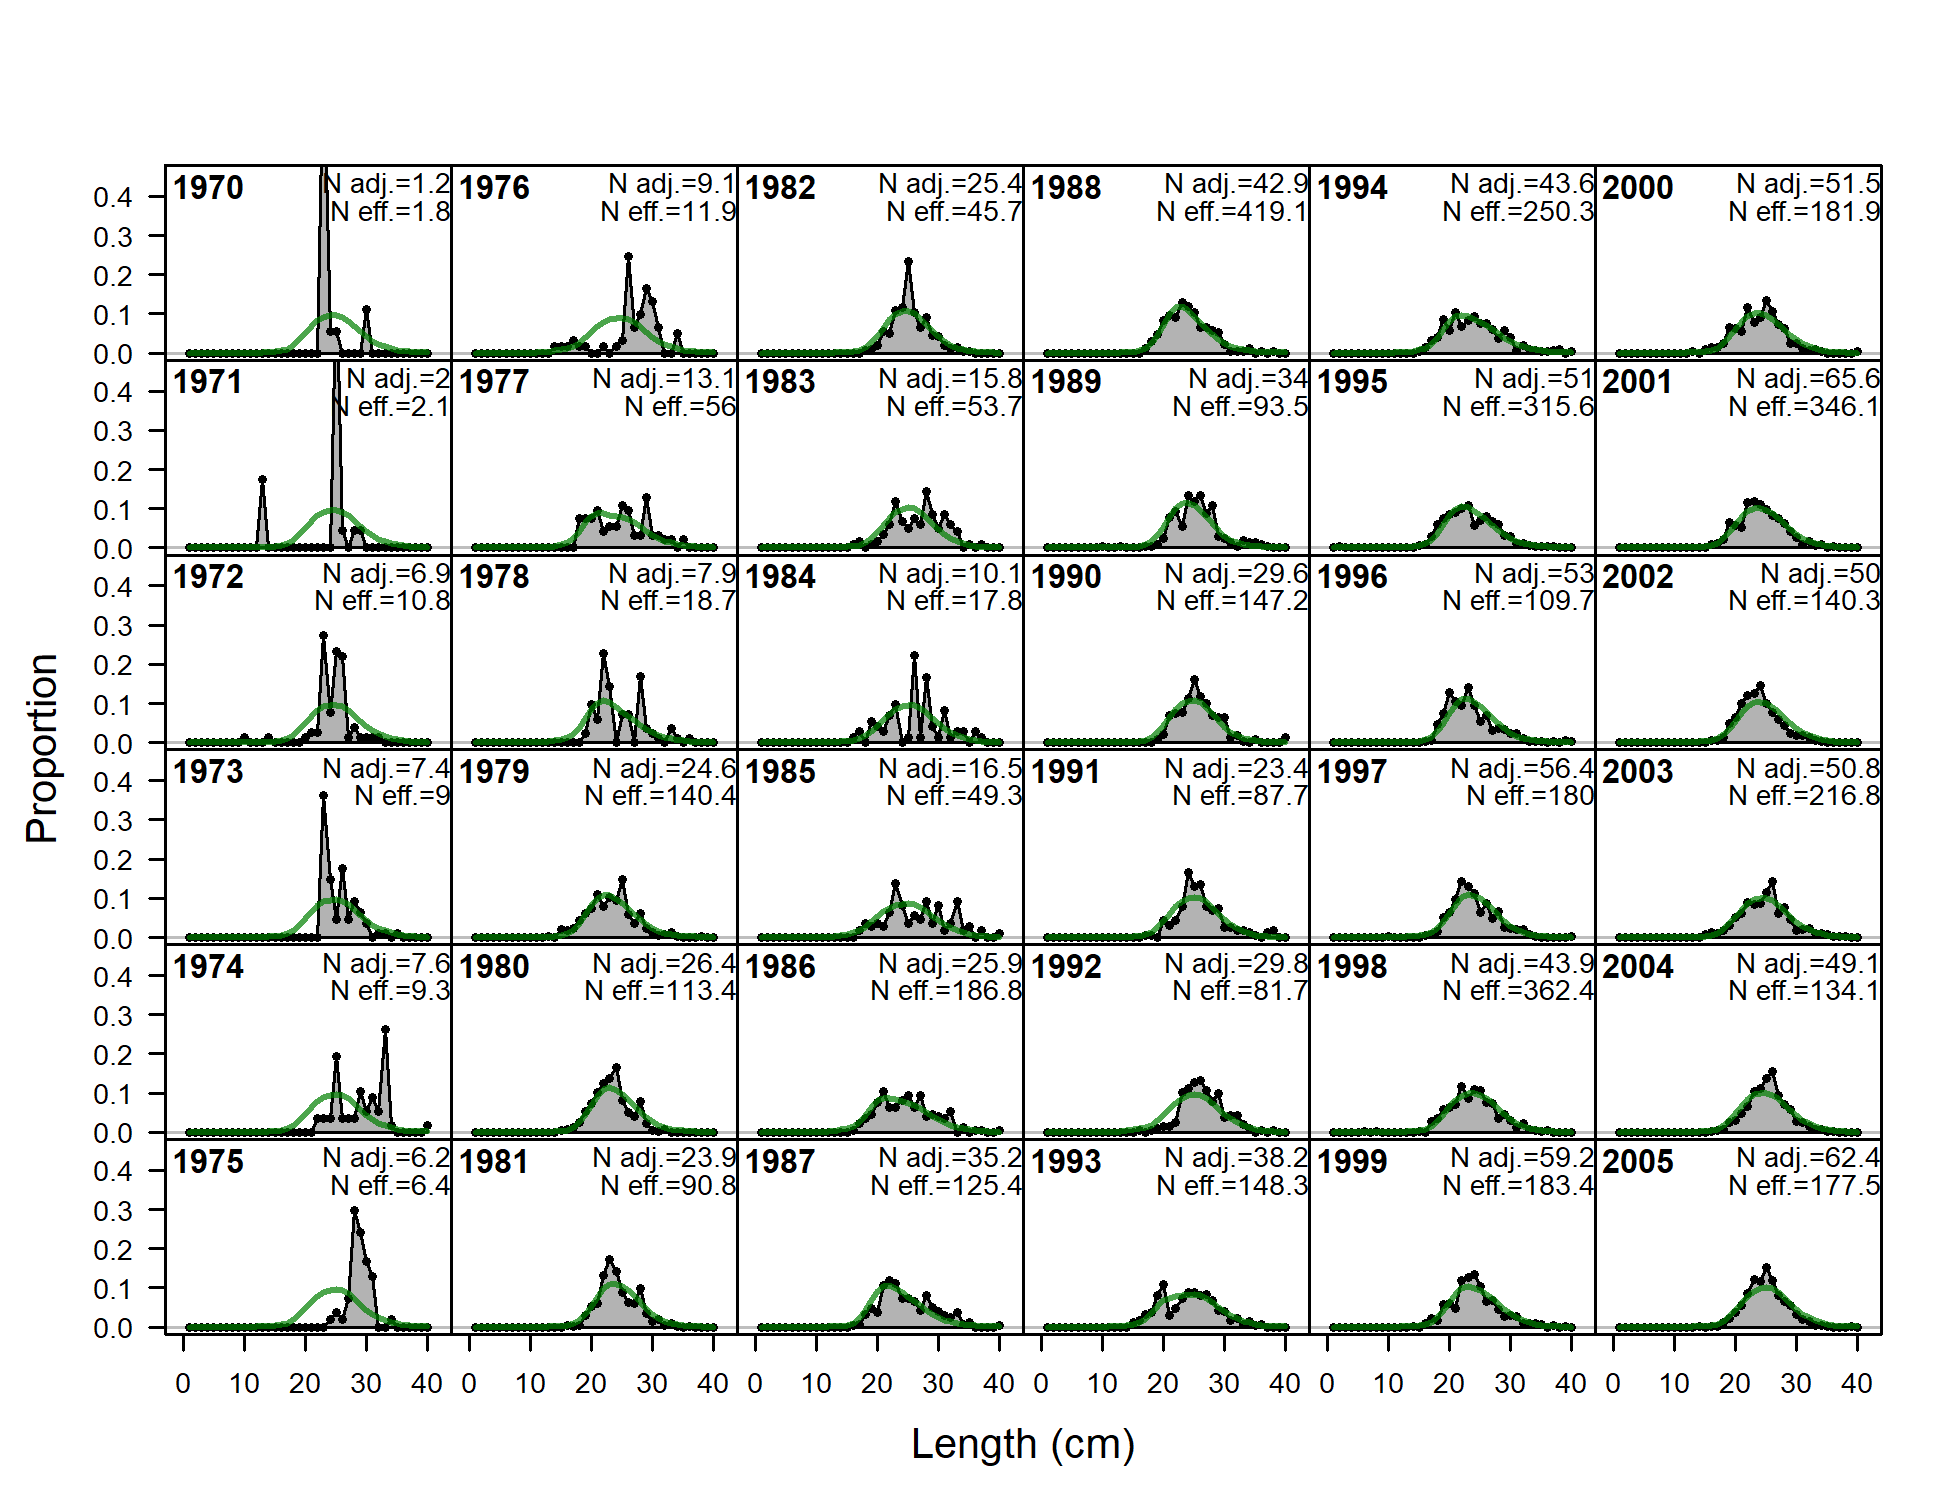
\includegraphics{./r4ss/plots_mod1/comp_lenfit_flt7mkt2_page1.png}

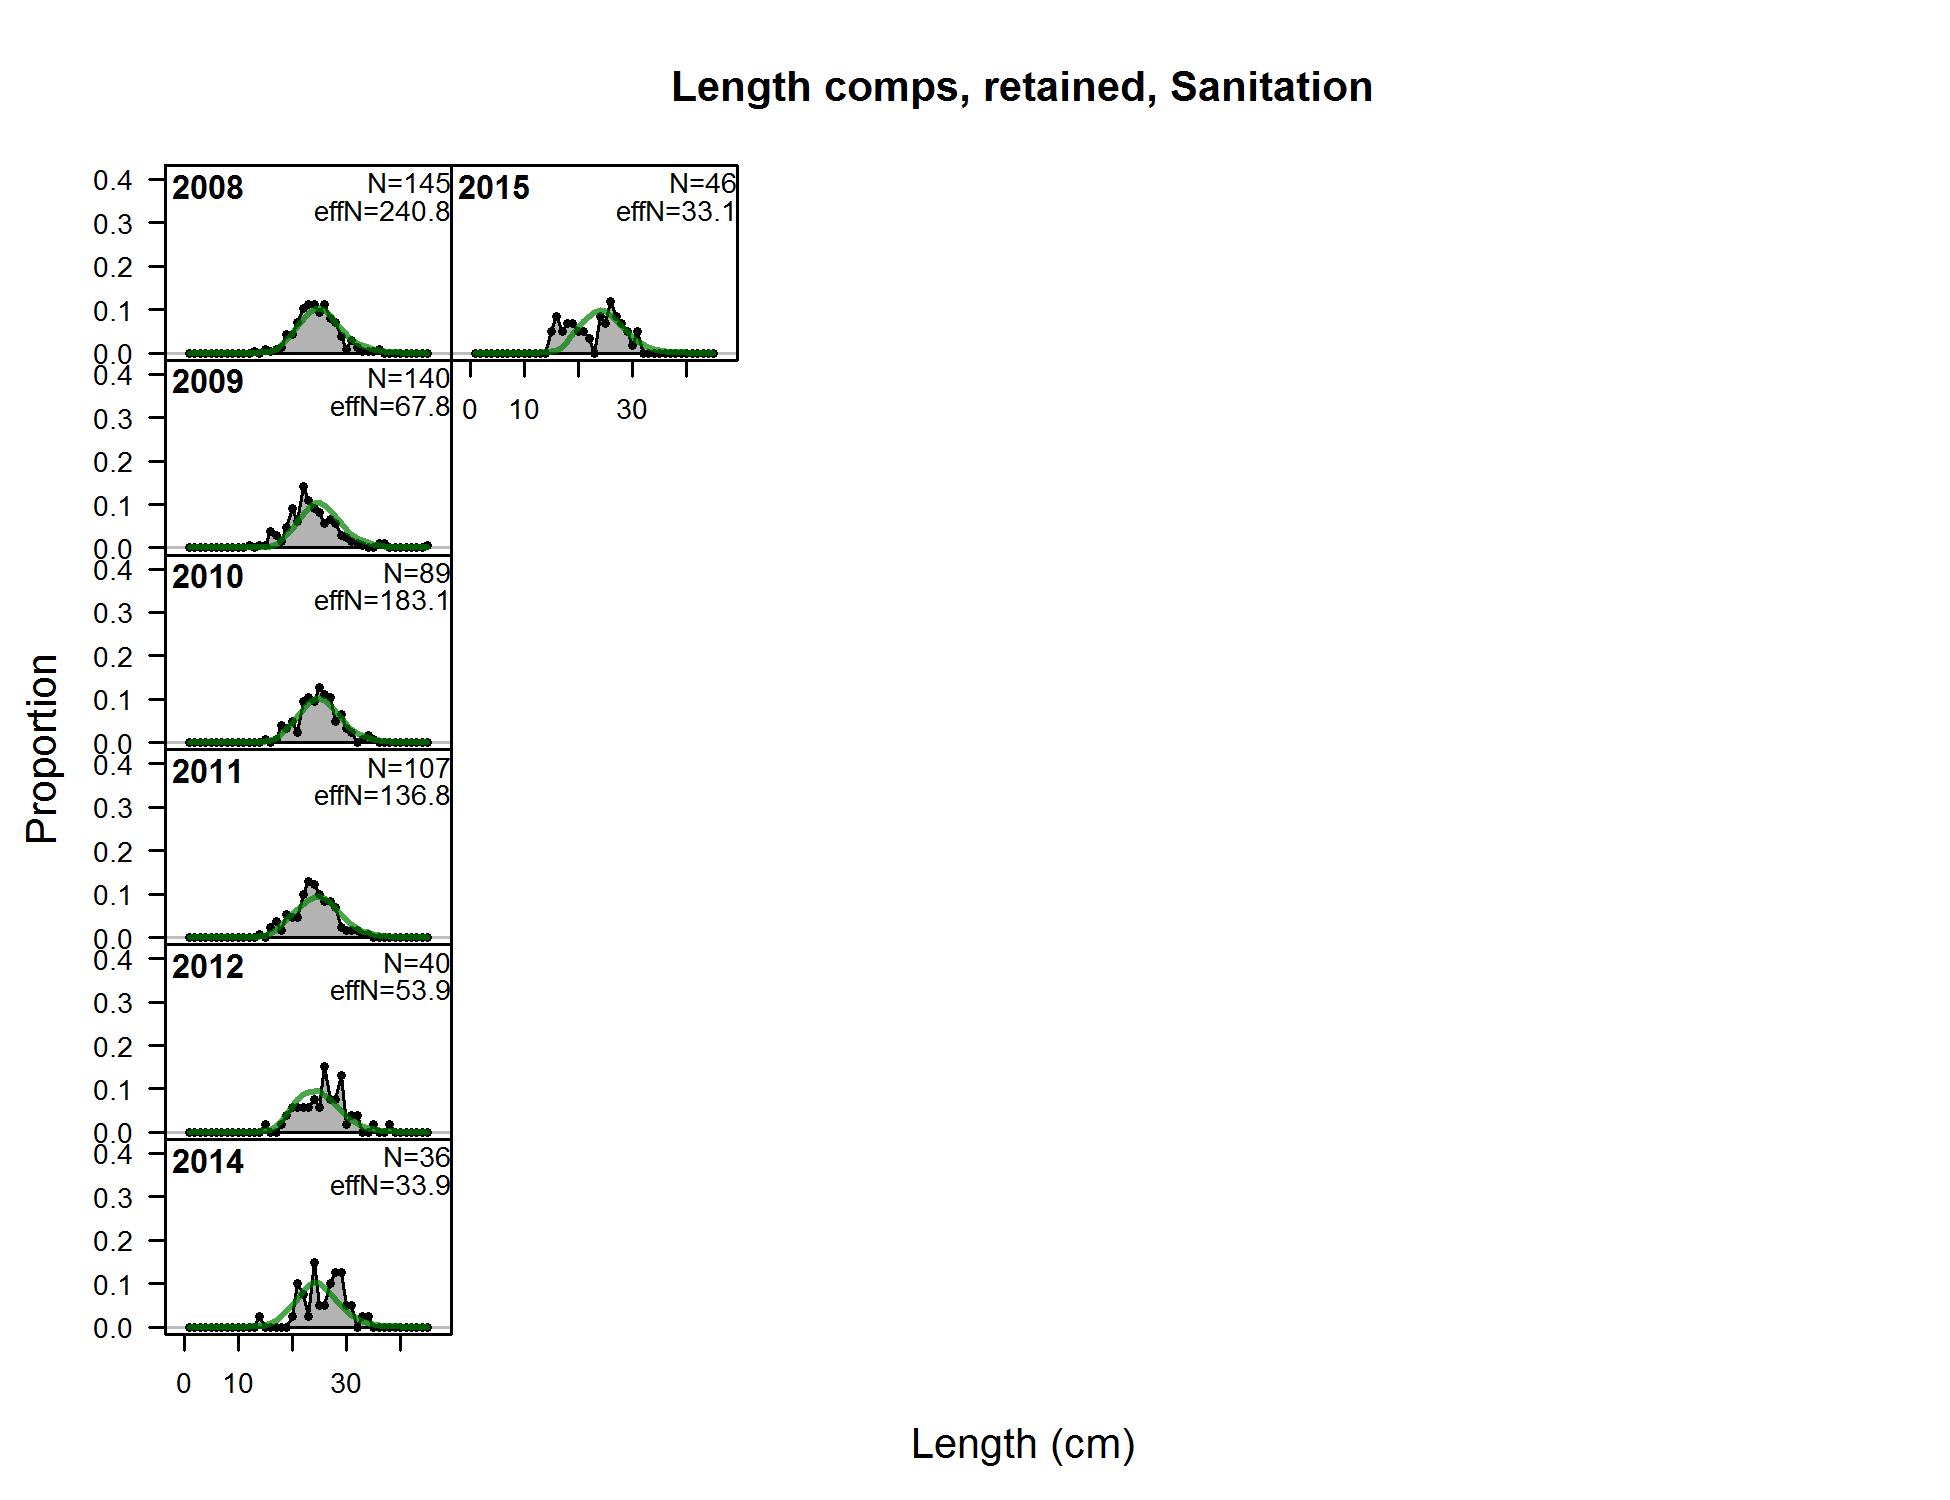
\includegraphics{./r4ss/plots_mod1/comp_lenfit_flt7mkt2_page2.png}

\begin{center} 

              Figure continued from previous page 

             \end{center}

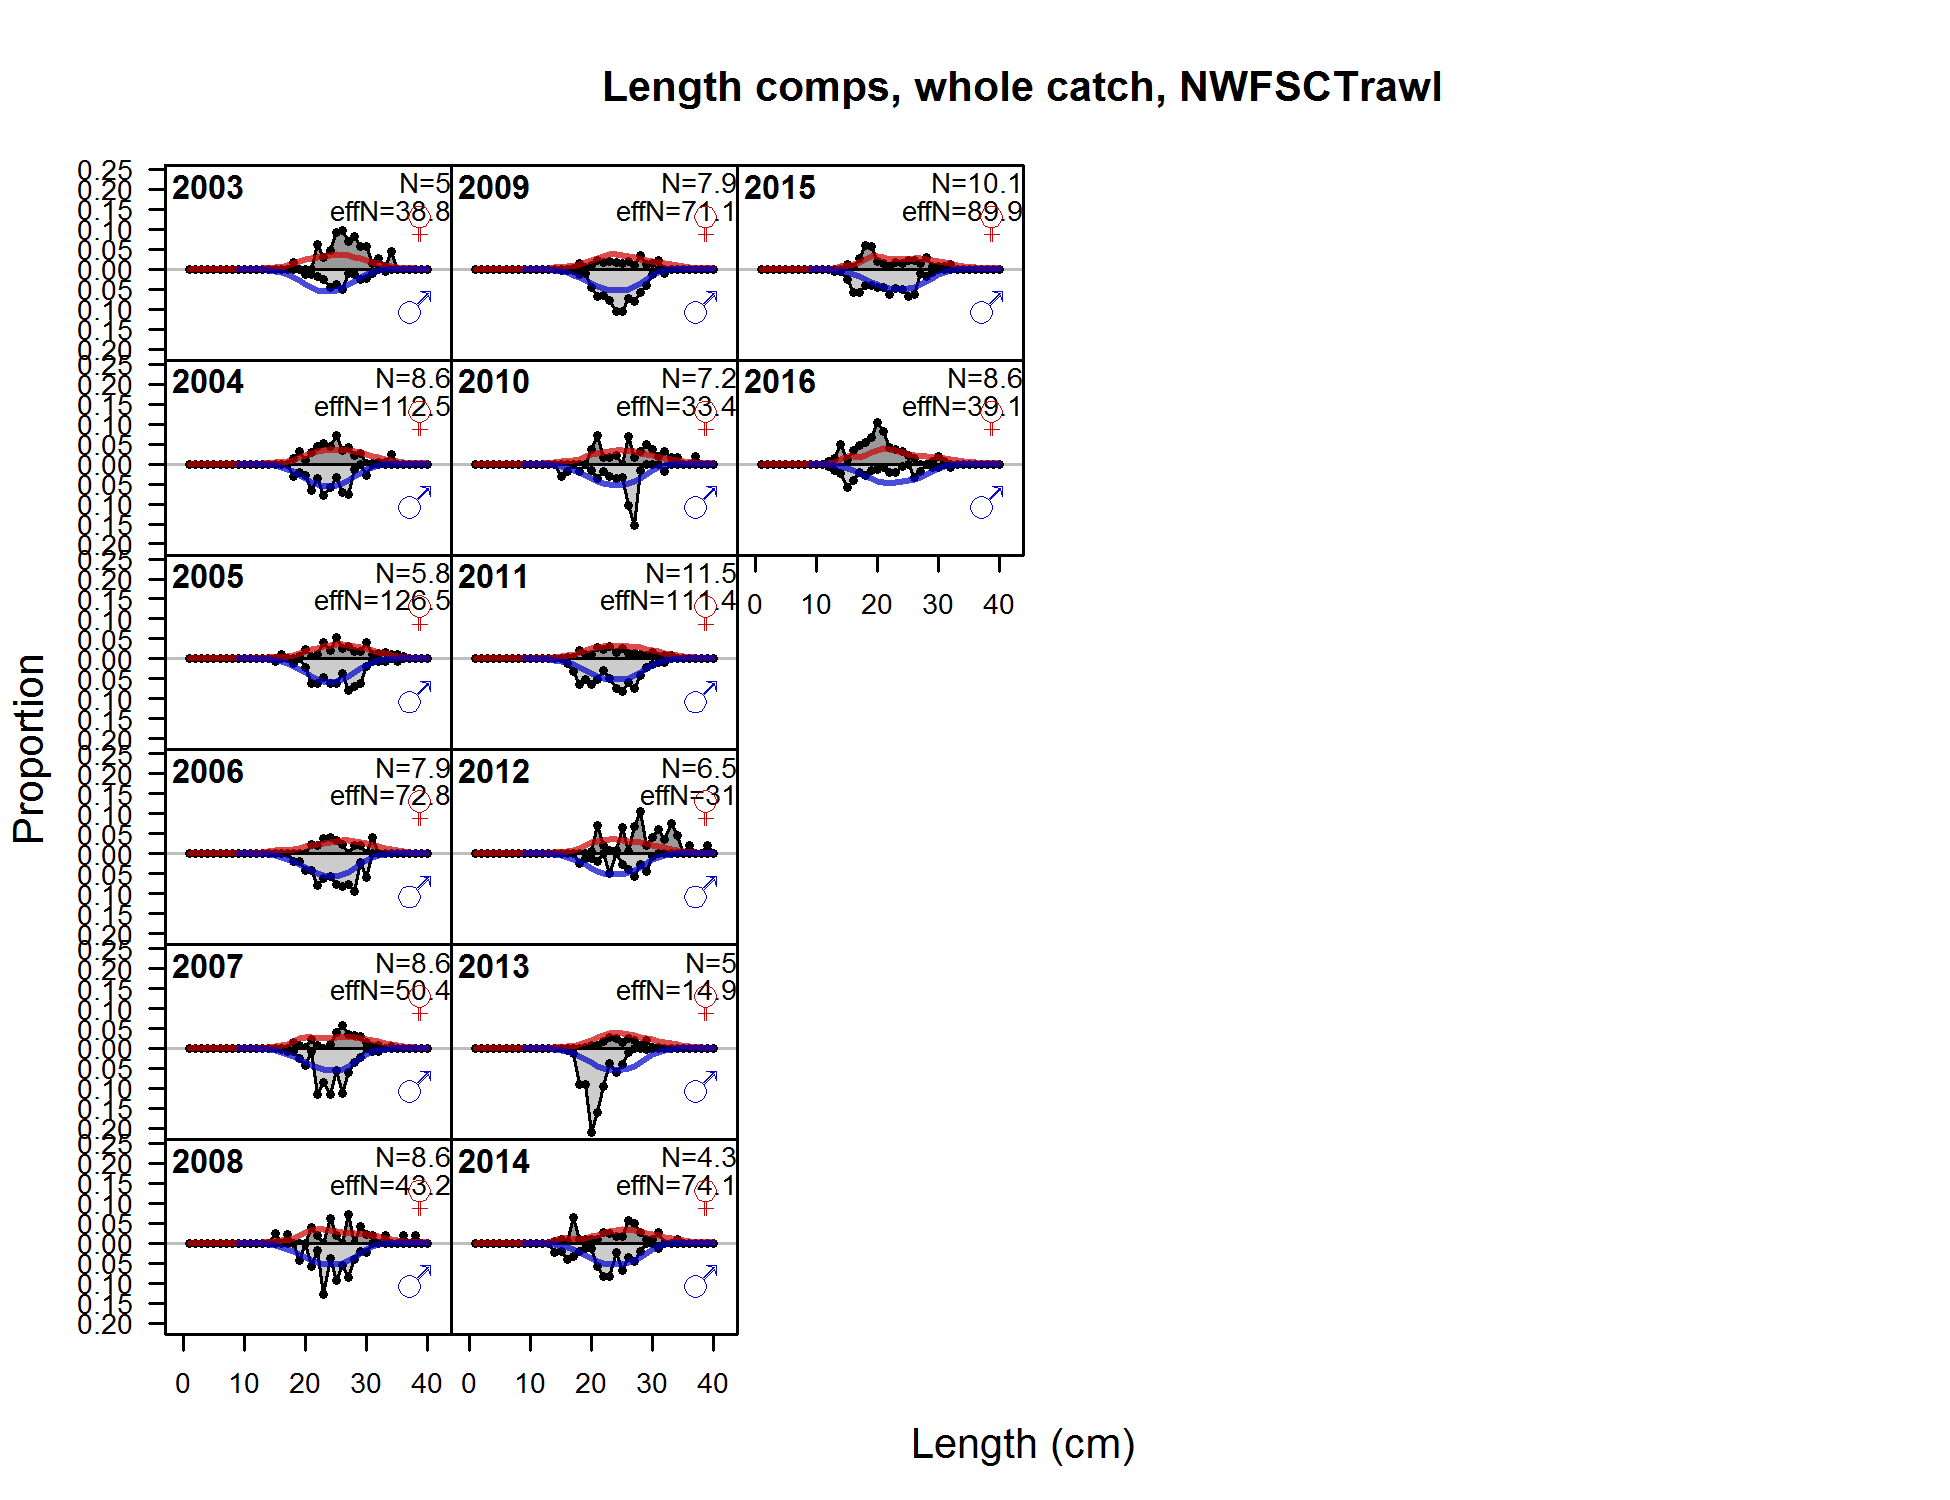
\includegraphics{./r4ss/plots_mod1/comp_lenfit_flt8mkt0.png}

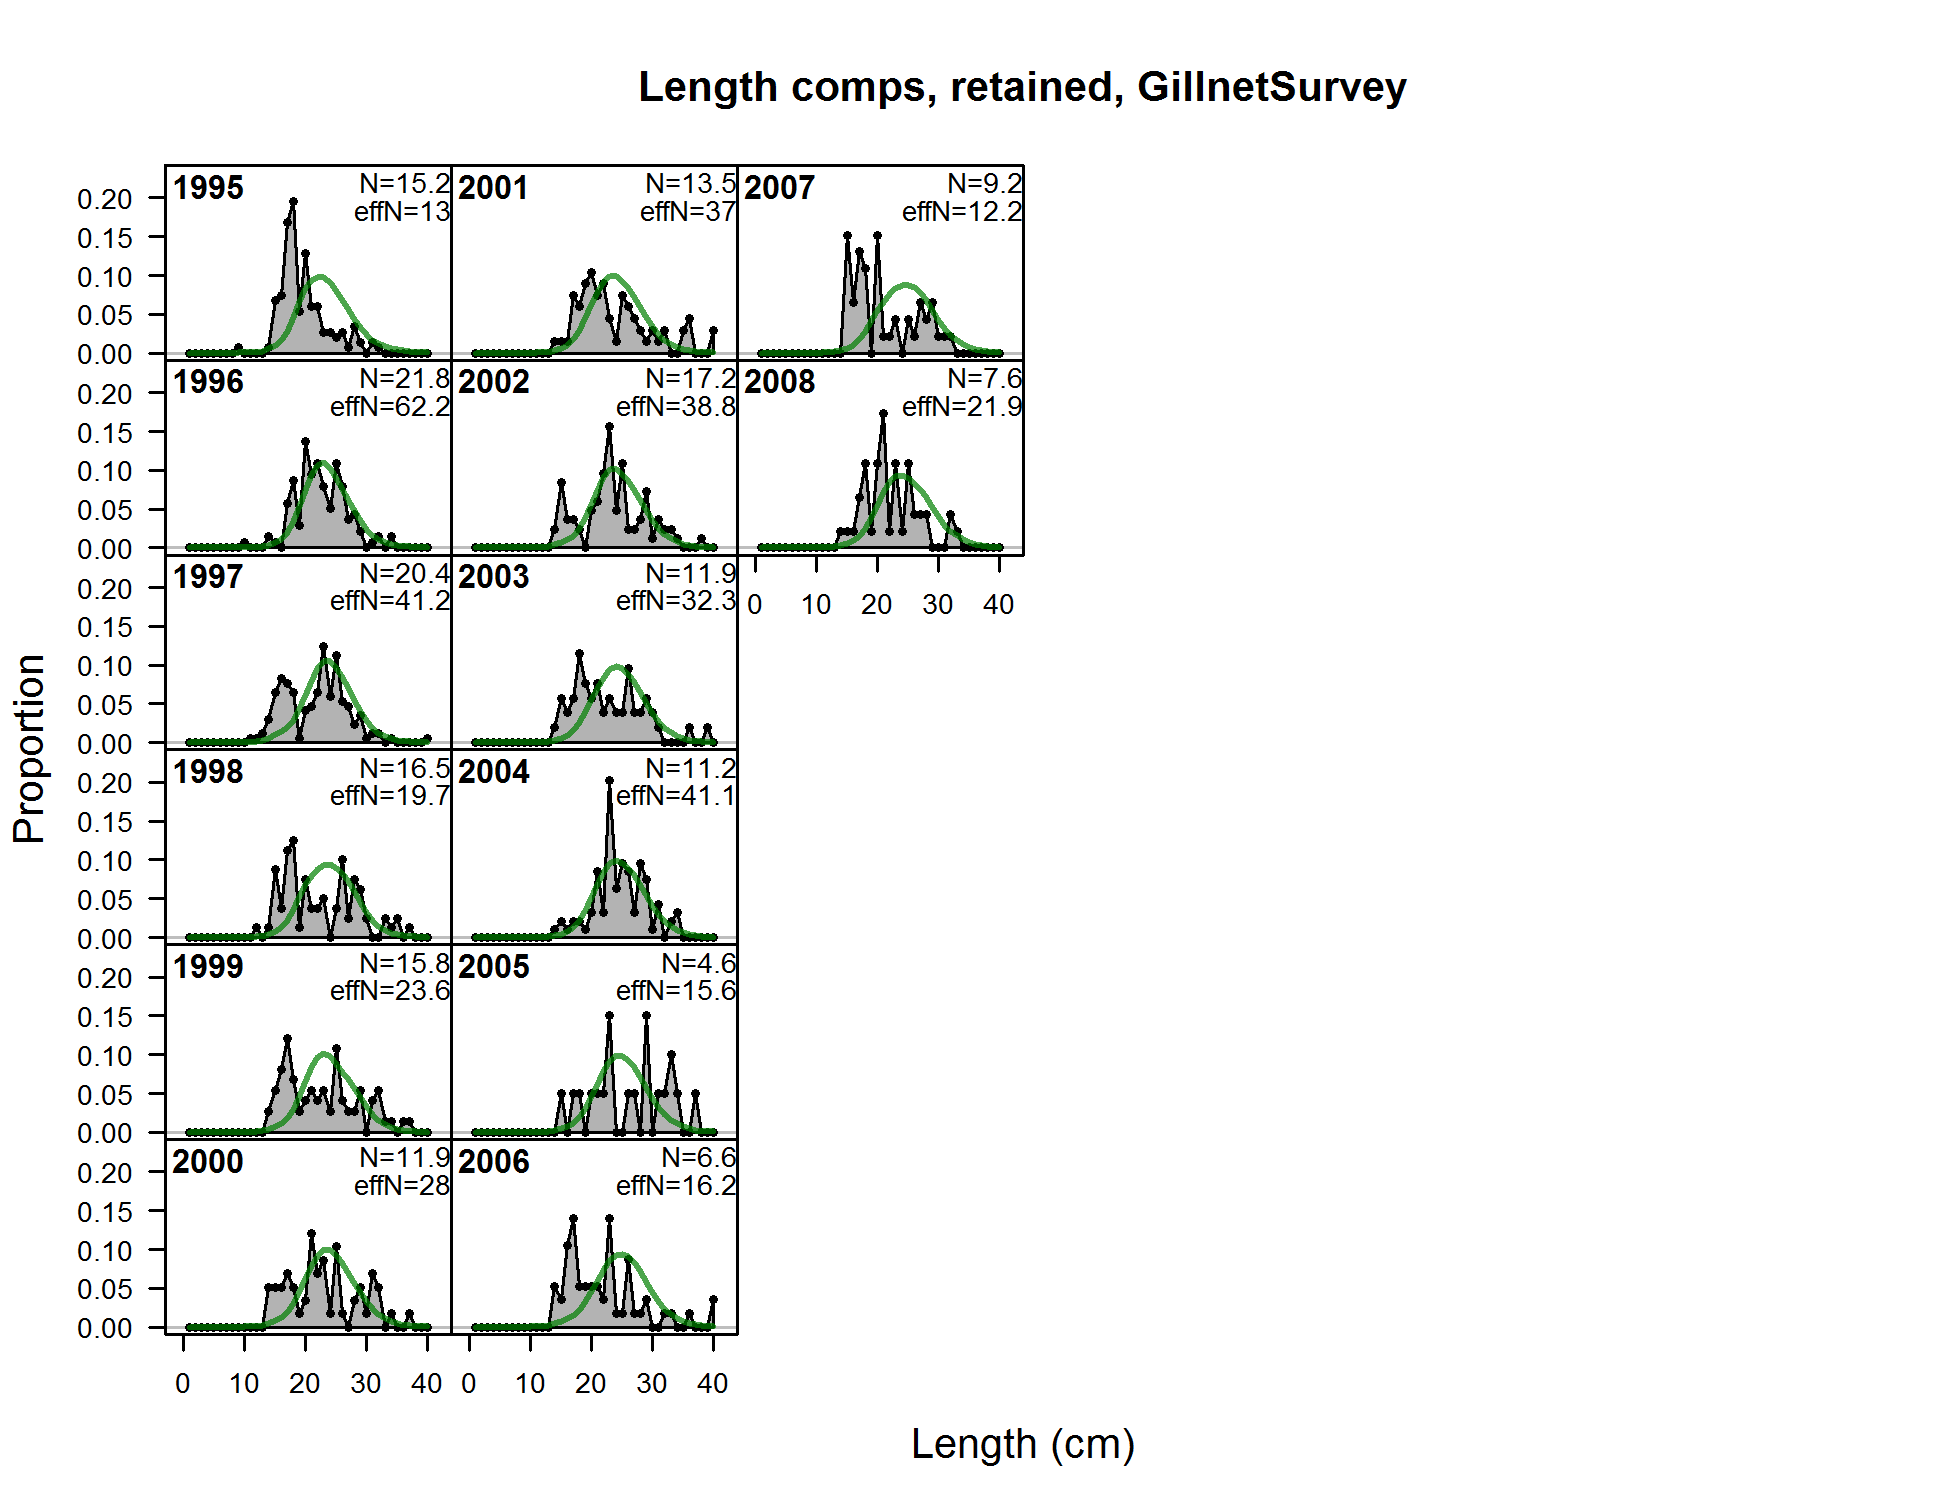
\includegraphics{./r4ss/plots_mod1/comp_lenfit_flt9mkt2.png}

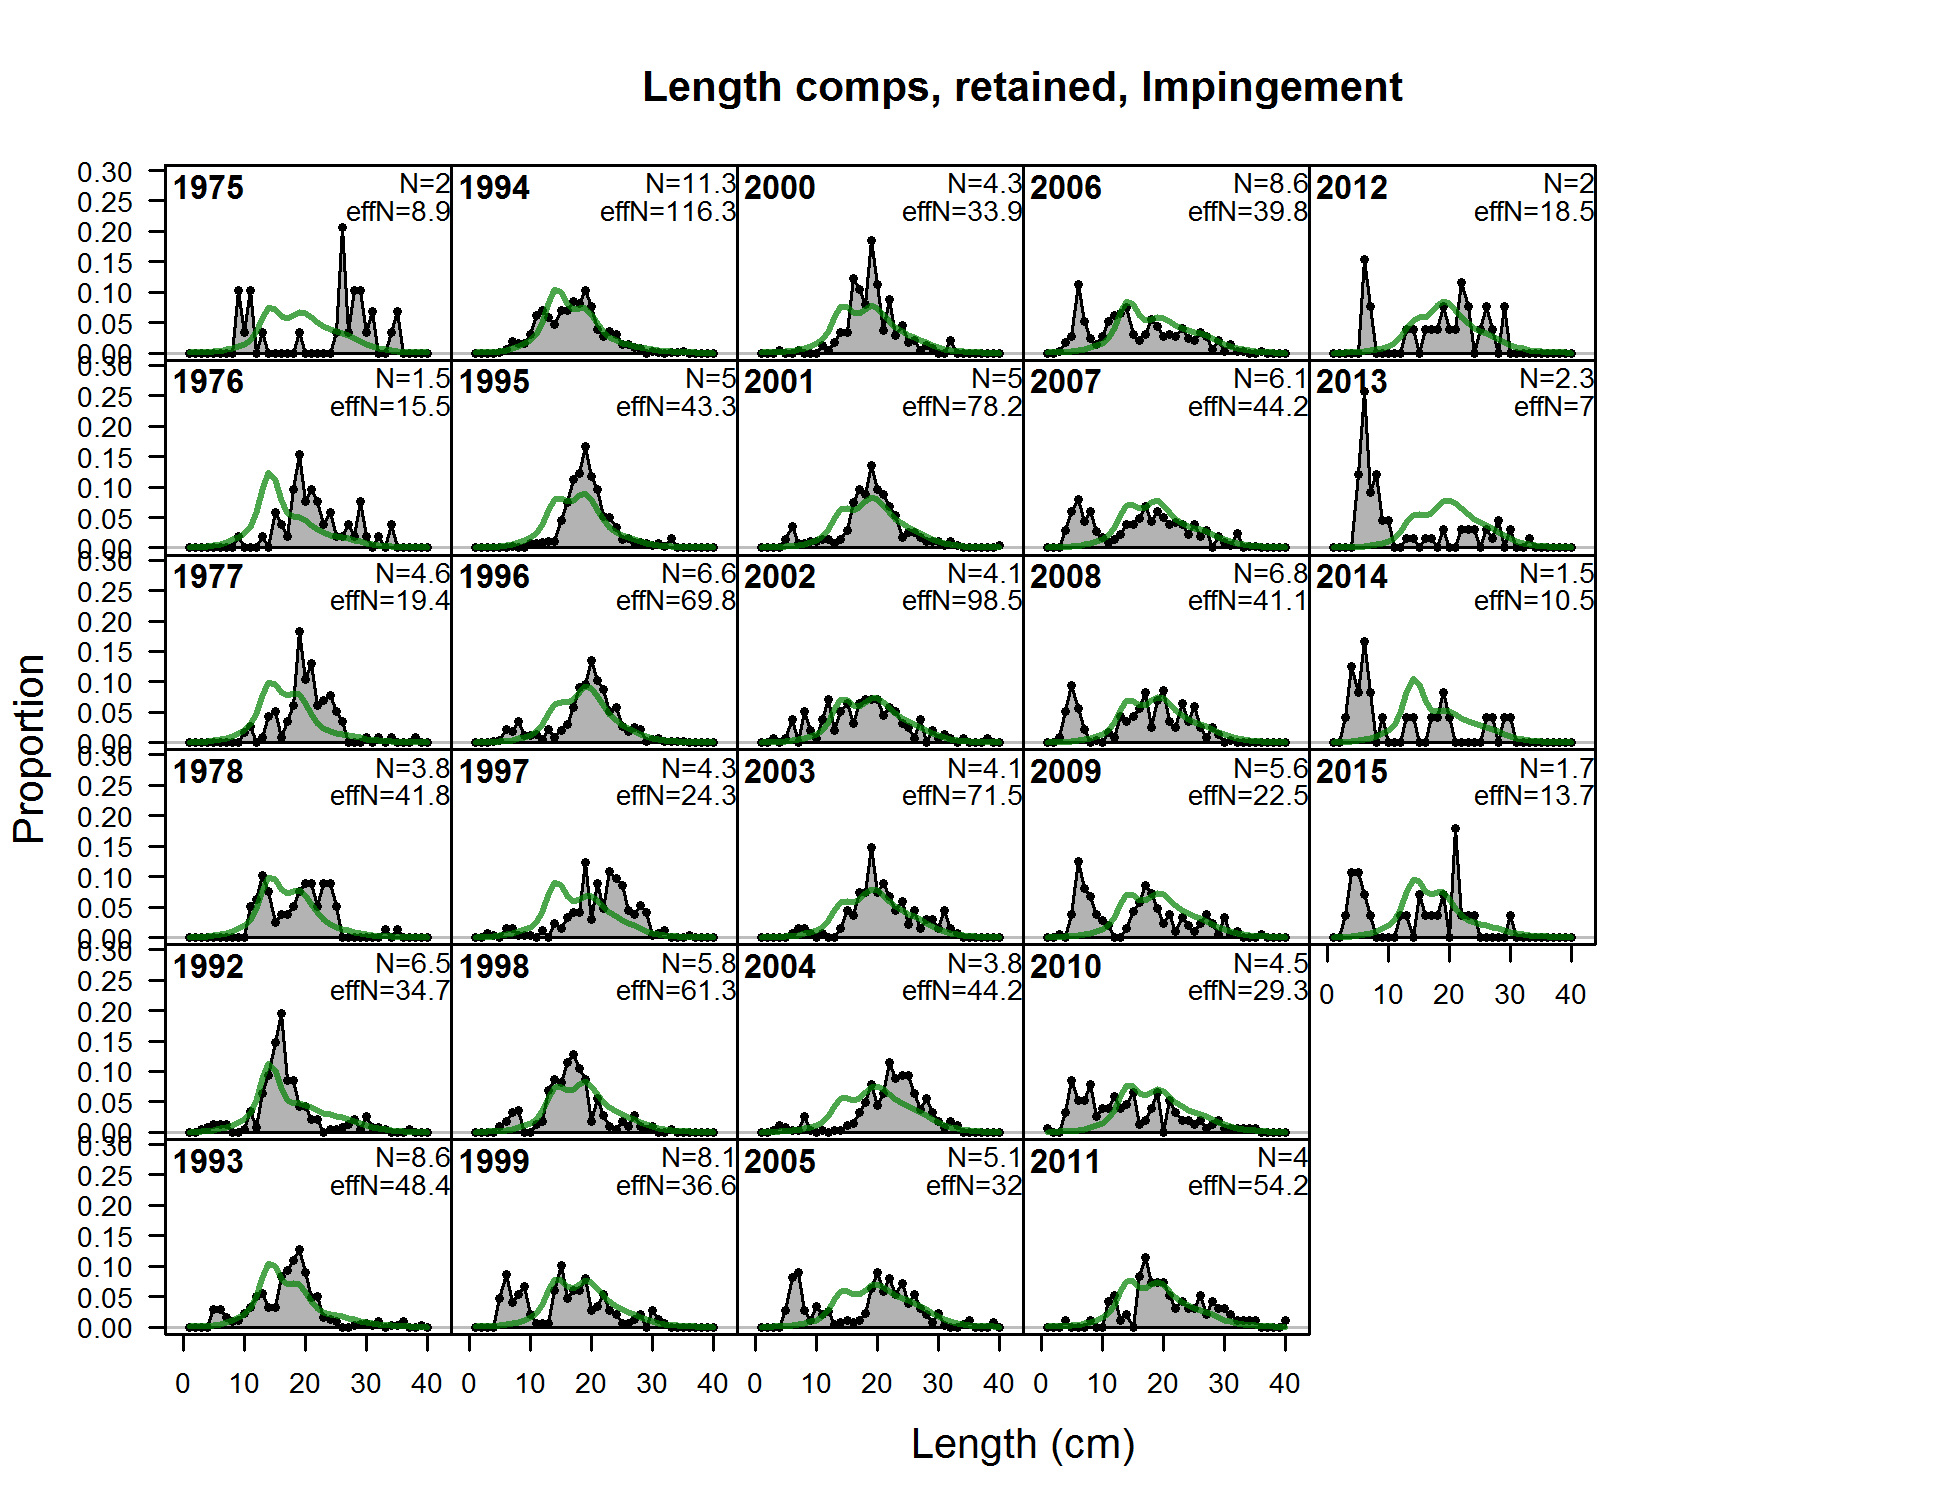
\includegraphics{./r4ss/plots_mod1/comp_lenfit_flt10mkt2.png}

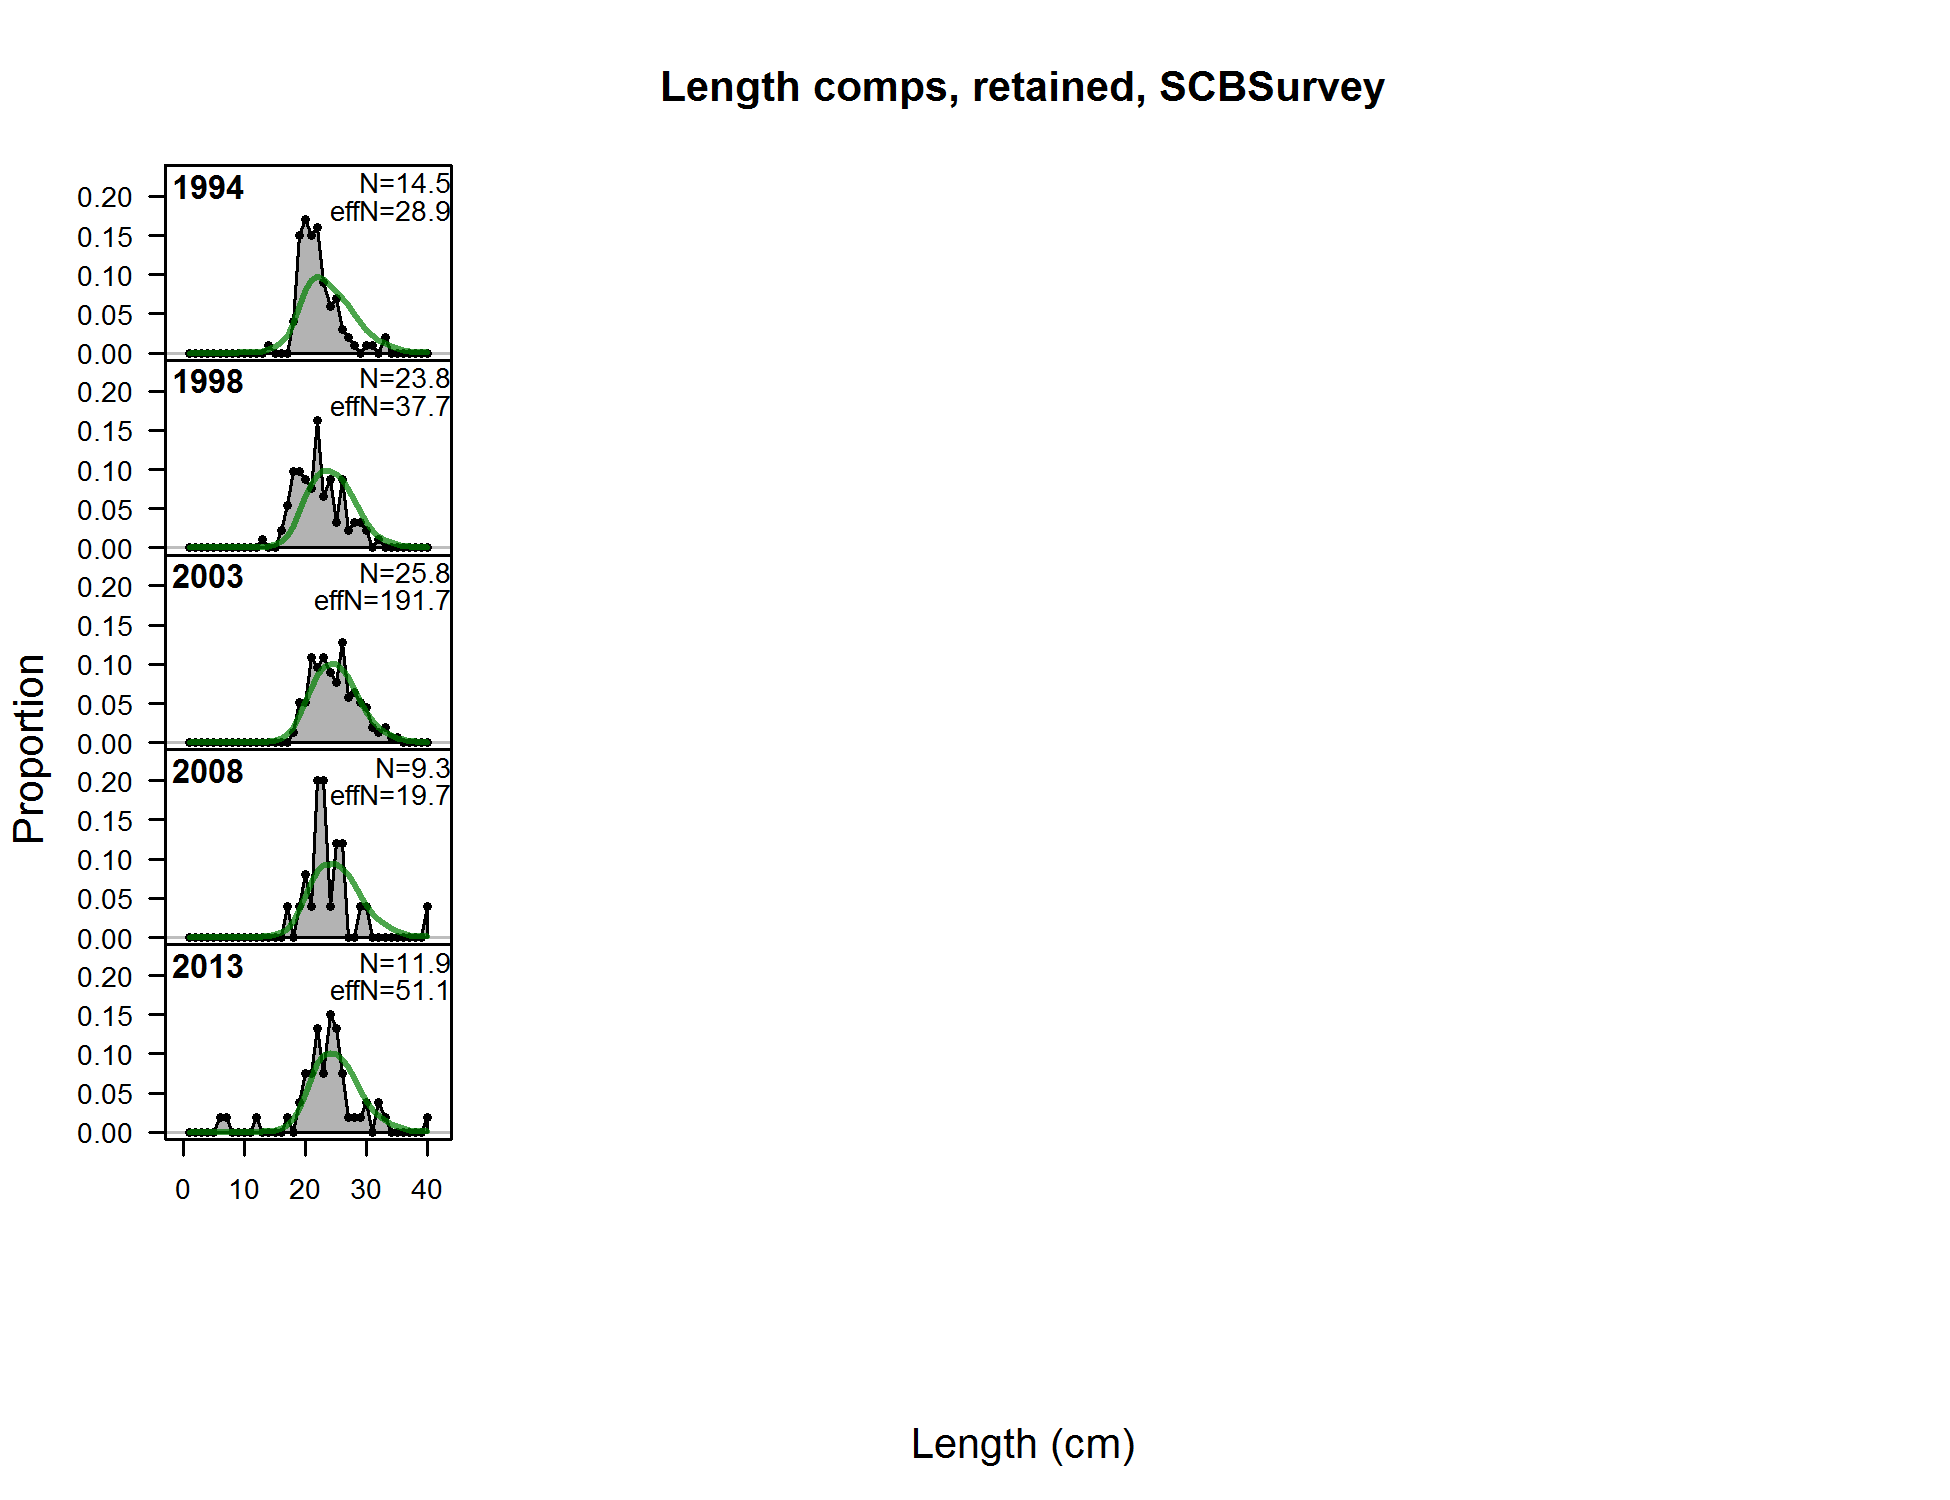
\includegraphics{./r4ss/plots_mod1/comp_lenfit_flt11mkt2.png}

\end{document}
